 \documentclass[11pt]{article}
% -----------------------------------------------------------------------------
% Response to the reviewers of MS CPENG-8674 (major revision, October 2026).
% Draft: answers are written only for the comments addressed so far.
% Code: MODULES/review29oct_fixed | Data: Data/06Nov_FINAL_SlabS10_7D_5sensors_5modes | Figures: ./figures_final
% Orange text = notes for the authors and placeholders (remove or fill before submission).
% -----------------------------------------------------------------------------
\usepackage[a4paper,margin=2.5cm]{geometry}
\usepackage{amsmath,amssymb,bm}
\usepackage{graphicx}
\usepackage{booktabs,multirow,array,longtable,tabularx}
\usepackage{xcolor}
\usepackage{caption,subcaption}
\usepackage{float}
\usepackage{enumitem}
\usepackage{titlesec}
\usepackage{tikz}
\usetikzlibrary{decorations.pathmorphing,arrows.meta,calc,positioning,patterns,decorations.pathreplacing,fit,backgrounds}
\usepackage[numbers,sort&compress]{natbib}
\usepackage[colorlinks=true,linkcolor=blue!50!black,citecolor=blue!50!black,urlcolor=magenta]{hyperref}

\definecolor{resp}{RGB}{25,70,170}
\definecolor{note}{RGB}{205,95,0}
\linespread{1.15}
\setlength{\parindent}{0pt}
\setlength{\parskip}{4pt}
\captionsetup{font=small,labelfont=bf,labelsep=colon}
\renewcommand{\thetable}{R\arabic{table}}
\renewcommand{\thefigure}{R\arabic{figure}}
\renewcommand{\theequation}{R\arabic{equation}}
\titleformat{\section}{\normalfont\large\bfseries}{}{0pt}{}
\titleformat{\subsection}{\normalfont\bfseries}{}{0pt}{}
\setlist{itemsep=1pt,topsep=2pt}

% --- Comment / response / action blocks (as in our previous response letters) ---
\newenvironment{rcomment}[1]{\par\bigskip\noindent\textbf{Comment\ifx&#1&\else\ #1\fi:}\ \itshape}{\par}
\newenvironment{response}{\par\smallskip\noindent\color{resp}\textbf{Response:}\ }{\par}
\newenvironment{action}{\par\smallskip\noindent\color{resp}\textbf{Action:}\ }{\par}
\newcommand{\pending}{\par\smallskip\noindent\textcolor{gray}{\textbf{Response:} \textit{pending --- this comment
has not been addressed yet.}}\par}
\newcommand{\authornote}[1]{\textcolor{note}{\textsf{[Authors: #1]}}}
\newcommand{\tbd}[1]{\textcolor{note}{\textsf{[#1]}}}
\newcommand{\lines}[1]{\tbd{lines #1}}

\newcommand{\m}{\mathbf{m}}
\newcommand{\z}{\mathbf{z}}
\newcommand{\f}{\mathbf{f}}

\begin{document}

\begin{center}
{\Large\bfseries Response to reviewer comments}\\[8pt]
\textbf{MANUSCRIPT ID:} CPENG-8674\\
\textbf{Date:} \today\\
\textbf{Title:} Uncertainty-aware damage identification in short-span bridges via physics-informed variational
autoencoder\\
\textbf{Journal:} Journal of Computing in Civil Engineering
\end{center}

%\noindent\fcolorbox{note}{note!6}{\parbox{\dimexpr\linewidth-2\fboxsep-2\fboxrule}{\small\color{note}\textsf{%
%\textbf{Draft status (\today).} Answers are given only for the comments addressed so far; the other comments are reproduced with the mark ``pending''. Orange text is for the authors: notes, and placeholders for the results of the
%training on the final dataset and for the line numbers of the revised manuscript. All numbers in blue come from the final dataset (\texttt{Data/06Nov\_FINAL\_SlabS10\_7D\_5sensors\_5modes}: bridge S10 of Moliner et al., 2017, as a beam on vertical elastic supports; five sensors, five modes) and the scripts in \texttt{MODULES/review29oct\_fixed} and
%\texttt{MODULES/baseline\_GaussCopula\_GaussMarginals}.}}}
%
%\bigskip
We would like to thank the three reviewers for the time and effort they devoted to conducting this insightful review.
In the following, we answer each comment point by point. 


%

% =============================================================================
\section{Reviewer \#1}
% =============================================================================
% The authors' notes on which these responses are based are kept in MODULES/_backup_09Nov_letter_user_notes/.

\begin{rcomment}{}
This paper presents a physics-informed Gaussian copula variational autoencoder for uncertainty-aware damage
identification using noisy natural frequencies and mode shapes. Replacing the learned decoder with a differentiable
eigensolver appears to be an interesting approach for end-to-end training, and the manuscript is clearly written. The work
builds on the authors' earlier Gaussian copula VAE (Reference 41) and extends it by embedding the eigensolver and
increasing the latent dimensionality from 2 to 5. The current validation is based on a single five-element synthetic
beam with measurement noise, and I believe that some additional evidence would further strengthen the conclusions
regarding uncertainty quantification, reliability, and scalability. Some clarifications are needed to better understand
the method and its applications.
\end{rcomment}

% -----------------------------------------------------------------------------
\begin{rcomment}{1}
The training and test data are generated using the same five-element model. Could the authors consider testing the trained model on observations generated from a finer mesh while retaining the same five damage zones and sensor locations as in the current paper? This would help assess robustness to model-form uncertainty, since field observations
may not necessarily be well represented by such a coarse discretization.
\end{rcomment}

\begin{response}
We have built a new, more realistic case study, which also addresses the concerns of Reviewer 2 (R2.2--R2.4). 
The bridge deck is discretized into $n_{e}  = 10$  Euler--Bernoulli beam elements and rests on elastic bearings, represented by vertical springs at both ends (see Fig.~\ref{fig:bridge}). 
The same five damage zones are considered along the deck, and two extra damage features are included for the stiffness of the bearings.  
We employ this 10-element parameterization to generate the training and validation data.
For the test dataset, we employ a finer discretization of the same structure, considering $n_{e} = 50$ elements along the bridge deck, with the same five damage zones, sensor locations, and design of experiments as the training data.
The instrumentation system is kept the same as in the original manuscript. 
%THIS GOES IN R2.
%The latent variables are one stiffness reduction factor per damage zone along the deck, as in the original submission, plus one stiffness factor per bearing (R2.2):
%\begin{equation}
%\hat{\mathbf{K}}_{\mathrm{G}}(\z)=\sum_{d=1}^{5} z_d\sum_{e\in\mathcal{Z}_d}\mathbf{K}_{e}
%+z_{b,L}\,\mathbf{K}_{b,L}+z_{b,R}\,\mathbf{K}_{b,R},
%\label{eq:Kz}
%\end{equation}
%where $\mathcal{Z}_d$ is the set of elements of zone $d$, and $\mathbf{K}_{b,L}$ and $\mathbf{K}_{b,R}$ contain the nominal stiffness of the left (L) and right (R) bearing springs.


%The test damage scenarios are also generated differently from the training ones (R1.5).
%The performance metrics of the identification on the testing dataset are reported in Table~\ref{tab:metricsB} (R1.3).
\end{response}

% -----------------------------------------------------------------------------
\begin{rcomment}{2}
The introduction identifies model uncertainty, measurement error, and environmental variability as sources of
ill-posedness, whereas the numerical study focuses primarily on measurement noise. It would be useful to investigate how
the proposed framework handles the other sources of uncertainty or, alternatively, to discuss this point more explicitly
as a limitation of the present study.
\end{rcomment}

\begin{response}
We have extended the case study to incorporate modeling error.
For that purpose, and responding also to R3.1, we have introduced a mass perturbation in the finite-element parameterization to account for discrepancies with respect to the nominal, reference properties of the system. 
The mass value of each structural element is independently perturbed as: 
\begin{equation}
	m_e^{\text{true}} = m_e^{\text{nom}} \left(1 + \epsilon \xi_e\right), \quad e = 1, \dots, n_{\text{e}},
	\label{eq:modeling_error}
\end{equation}
where $m_e^{\text{nom}}$ denotes the nominal mass value at the $e$-th element, with $n_{e}$ total elements; $\xi_e$ is an independent sample from a standard Gaussian random variable; and $\epsilon$ is the model-error level. 
In this work, we assign $\epsilon = 0.05$ to represent a $5\%$ error. 
To incorporate this discrepancy, we employ the perturbed values to generate the datasets (observations), while the nominal values are fed as known properties into the physics-informed VAE architecture. 
Besides, the use of a coarse mesh (10 elements) for training compared to that used for testing (50 elements), as requested in R1.1, introduces the effect of discretization error.

A realistic description of environmental and operational effects requires long-term monitoring data, which cannot be reproduced reliably in the current synthetic dataset. 
We now specify in the introduction the sources of uncertainty handled in the present work. 
In the conclusions, we describe in more detail the limitations of the methodology, and acknowledge the lack of environmental variability, which is left for future work as part of the experimental validation. 


%
%We agree that measurement noise is not the only source of uncertainty in practice. The revised study accounts for the
%following sources:
%\begin{enumerate}[leftmargin=*,label=(\alph*)]
%\item \emph{Measurement error.} As in the original submission, the natural frequencies and mode shapes are corrupted
%with Gaussian noise (2.5\% of the frequencies and 5\% of the peak amplitude of the mode shapes).
%\item \emph{Modelling error.} The data are generated with a model that differs from the one used by the SciML method. The
%mass of each 1~m segment of every simulated structure is perturbed as
%\begin{equation}
%\mathbf{M}_e^{\mathrm{data}}=(1+\mu_{s(e)})\,\mathbf{M}_e,\qquad \mu_{s}\sim\mathcal{N}(0,0.05^2),
%\label{eq:asbuilt}
%\end{equation}
%where $s(e)$ is the segment of element $e$, whereas the decoder keeps the nominal mass matrix. Uncertain permanent loads are
%also considered in dynamic studies of short-span bridges (e.g., $\pm30\%$ of the ballast thickness in Moliner et al.,
%2017). In addition, the test data are generated with a finer discretization (50 elements, R1.1) to explore the robustness
%against model-form error.
%\item \emph{Limited information.} We also explore the effect of a scarce measurement data by reducing the number of identified modes (three instead of five), as also requested by Reviewer 3 (R3.4).
%\item \emph{Environmental and operational variability.} A realistic description of these effects requires long-term
%monitoring data, which cannot be reproduced reliably in a synthetic dataset. We acknowledge this as a limitation of the
%present validation and propose an experimental validation that incorporates this source of uncertainty as future work.
%\end{enumerate}

%The statistics of the measurement and modelling errors are estimated by simulation and included in the likelihood (R1.3).
%Note that the objective of the present work is not to disentangle these sources of uncertainty (i.e., to quantify the  contribution of each one), which could be addressed in future work, but to include them to offer a realistic case study
%and a reliable validation.
\end{response}

%\begin{action}
%New paragraph on the sources of uncertainty \lines{xx--yy}, with Eq.~\tbd{x} (Eq.~\eqref{eq:asbuilt}); environmental
%and operational variability discussed as a limitation in the conclusions \lines{xx--yy}.
%\end{action}

% -----------------------------------------------------------------------------
\begin{rcomment}{3}
The abstract reports 77.2\% coverage (line 32), whereas line 352 reports a value of 0.789 for nominal 95\% intervals.
Could the authors clarify how these two values are related? A value below 80\% for nominal 95\% intervals may indicate
some undercoverage. A brief discussion of how the uncertainty intervals are calibrated would therefore be helpful.
\end{rcomment}
\begin{response}
We have entirely updated the results section according to the new case study and the corresponding train/validation/test datasets. 
We must also mention that there was an error in the calculation of the $95\%$ coverage in the submitted version, which produced the undercoverage results. 
In the updated manuscript, we now include (Section entitled ``Results and discussion'') the detailed formulation of the performance metrics and a dedicated table with the obtained results. 
	
\textcolor{red}{[This can be removed here and only included in paper:]} For each observation $\m_t$ ($t=1,\dots,N_{\text{test}}$) of the test dataset, with true damage condition
$\z^{\text{true}}_t\in[z_{\text{lb}},z_{\text{ub}}]^{D}$, the trained encoder (weights $\bm{\theta}^{*}$) provides the parameters $\bm\zeta_{\bm{\theta}^{*}}$ of the approximate posterior $q_{\bm\zeta_{\bm{\theta}^{*}}}(\z|\m_t)$ (Eq.~(8) of the manuscript). The marginal $q_{t,d}$ of each component $d=1,\dots,D$ is a truncated normal distribution: $z_d$ follows a Gaussian distribution with mean $\mu_{t,d}(\bm{\theta}^{*})$ and standard deviation $\sigma_{t,d}(\bm{\theta}^{*})$, truncated to $[z_{\text{lb}},z_{\text{ub}}]$. 
For notational simplicity, from now on we omit the dependence of the distribution parameters on $\bm{\theta}^{*}$. 
The density and cumulative distribution function
(CDF) of this truncated Gaussian are:
\begin{equation}
	q_{t,d}(z)=\frac{\varphi\big((z-\mu_{t,d})/\sigma_{t,d}\big)}{\sigma_{t,d}\,Z_{t,d}},\qquad
	F_{t,d}(z)=\frac{\Psi\big((z-\mu_{t,d})/\sigma_{t,d}\big)-\Psi(\alpha_{t,d})}{Z_{t,d}},\qquad
	z\in[z_{\text{lb}},z_{\text{ub}}],
	\label{eq:marginal_tn}
\end{equation}
where $\varphi$ and $\Psi$ are the standard normal PDF and CDF, $\alpha_{t,d}=(z_{\text{lb}}-\mu_{t,d})/\sigma_{t,d}$,
$\beta_{t,d}=(z_{\text{ub}}-\mu_{t,d})/\sigma_{t,d}$, and $Z_{t,d}=\Psi(\beta_{t,d})-\Psi(\alpha_{t,d})$. %Every metric is averaged over the $N_{\text{test}}\times D$ stiffness factors of the test dataset:
The metrics, averaged over the test dataset, are calculated as follows:
\begin{itemize}[leftmargin=*]
	\item \emph{Mean squared error (MSE) and mean absolute error (MAE)} of the point estimate $\hat z_{t,d}$, the mean of
	the marginal posterior of Eq.~\eqref{eq:marginal_tn}, which has a closed form:
	\begin{equation*}
		\hat z_{t,d}=\int_{z_{\text{lb}}}^{z_{\text{ub}}} z\,q_{t,d}(z)\,\mathrm{d}z
		=\mu_{t,d}+\sigma_{t,d}\,\frac{\varphi(\alpha_{t,d})-\varphi(\beta_{t,d})}{Z_{t,d}},
	\end{equation*}
	\begin{equation}
		\mathrm{MSE}=\frac{1}{N_{\text{test}}D}\sum_{t=1}^{N_{\text{test}}}\sum_{d=1}^{D}\big(\hat z_{t,d}-z^{\text{true}}_{t,d}\big)^2,\qquad
		\mathrm{MAE}=\frac{1}{N_{\text{test}}D}\sum_{t=1}^{N_{\text{test}}}\sum_{d=1}^{D}\big|\hat z_{t,d}-z^{\text{true}}_{t,d}\big|.
		\label{eq:mse_mae}
	\end{equation}
	\item \emph{Average log-likelihood (ALL)} of the true values under the marginal posteriors:
	\begin{equation}
		\mathrm{ALL}=\frac{1}{N_{\text{test}}D}\sum_{t=1}^{N_{\text{test}}}\sum_{d=1}^{D}\log q_{t,d}\big(z^{\text{true}}_{t,d}\big).
		\label{eq:all}
	\end{equation}
	\item \emph{Coverage}: fraction of the true values that lie inside the central credible interval of level $p$, i.e.,
	between the $(1-p)/2$ and $(1+p)/2$ quantiles of the marginal posterior:
	\begin{equation}
		C(p)=\frac{1}{N_{\text{test}}D}\sum_{t=1}^{N_{\text{test}}}\sum_{d=1}^{D}\mathbb{I}\Big[\frac{1-p}{2}\le F_{t,d}\big(z^{\text{true}}_{t,d}\big)\le\frac{1+p}{2}\Big],
		\label{eq:coverage}
	\end{equation}
	where $\mathbb{I}[\cdot]$ equals 1 if the condition holds, and 0 otherwise. The 95\% coverage is $C(0.95)$. If the
	posterior is calibrated, $C(p)\approx p$; a lower value (undercoverage) means that the true values fall outside the
	intervals more often than their level indicates.
	\item \emph{Mean absolute calibration error (MACE)} over $n_l=19$ levels $p_l=0.05,0.10,\dots,0.95$:
	\begin{equation}
		\mathrm{MACE}=\frac{1}{n_l}\sum_{l=1}^{n_l}\big|C(p_l)-p_l\big|.
		\label{eq:mace}
	\end{equation}
\end{itemize}
%	The credible intervals are not recalibrated after training: they are the central quantiles of the marginal posteriors
%	predicted by the VAE, and Eqs.~\eqref{eq:coverage} and \eqref{eq:mace} evaluate their calibration.

%	In the submitted version, due to a programming error, the 95\% coverage was computed as
%	\begin{equation*}
%		C_{\text{submitted}}=\frac{1}{N^2D}\sum_{t=1}^{N}\sum_{t'=1}^{N}\sum_{d=1}^{D}
%		\mathbb{I}\big[\mu_{t,d}-1.96\,\sigma_{t,d}\le z^*_{t',d}\le\mu_{t,d}+1.96\,\sigma_{t,d}\big],
%	\end{equation*}
%	i.e., the interval of each test observation $t$ was evaluated at the true values $z^*_{t',d}$ of all the $N$ test
%	observations, instead of only at its own true values ($t'=t$) as in Eq.~\eqref{eq:coverage}. Besides,
%	$\mu_{t,d}\pm1.96\,\sigma_{t,d}$ are the bounds of the 95\% interval of the Gaussian distribution before its
%	truncation to $[z_{\text{lb}},z_{\text{ub}}]$, whereas Eq.~\eqref{eq:coverage} uses the quantiles of the truncated
%	distribution.
Table~\ref{tab:metricsB} reports the metrics on the test dataset. 
%Overall, 87.8\% of the true stiffness factors lie inside their 95\% credible intervals and the MACE is 0.112. 
%The table separates the stiffness factors with intermediate or mild damage ($z^*<0.80$) from the healthy ones and those with light damage ($z^*\ge0.80$). 
%A loss of stiffness below 20\% in
%one zone changes the natural frequencies by about as much as their identification noise or less (R1.6), so the latter are hard to distinguish from each other. The 95\% credible intervals are well calibrated for this second group (coverage	of 0.885) and somewhat too narrow for the damaged factors (0.854), for which the point estimate is also less accurate (MAE of 0.072 against 0.063).
	
	\begin{table}[H]
		\centering\small
		\caption{Performance metrics, Eqs.~\eqref{eq:mse_mae}--\eqref{eq:mace}, on the test dataset.}
		\label{tab:metricsB}
		\begin{tabular}{lc}
			\toprule
			Metric & Test dataset \\
			\midrule
			MSE & 0.00570 \\
			MAE & 0.0601 \\
			ALL & 1.723 \\
			95\% coverage, $C(0.95)$ & 0.900 \\
			MACE & 0.101 \\
			\bottomrule
		\end{tabular}
	\end{table}
\end{response}


%

% -----------------------------------------------------------------------------
\begin{rcomment}{4}
References 39 (Gaussian mixture autoencoder) and 41 (Gaussian copula VAE) introduce closely related methods that could
potentially serve as useful baselines. A comparison with these approaches would help assess the benefits of the proposed
strategy more effectively.
\end{rcomment}

\begin{response}
The proposed method builds on two previous works of the authors: the Gaussian mixture autoencoder of Ref.~\cite{Navamuel_wes2025} (Ref.~39 of the manuscript) and the Gaussian copula VAE of Ref.~\cite{Arxiv_Navamuel2026copula2d} (Ref.~41 of the manuscript).
In both works, rather than being solved exactly, the forward operator is approximated by an additional neural network (decoder) that acts as a surrogate. 
This approach requires a two-step training strategy, where the approximate forward model (surrogate) is first trained independently. 
In the second step, the VAE is trained to find the optimal encoder weights while keeping the decoder weights frozen from the previous step. 
This approach provided good results in our previous works. 
However, it increases the number of trainable parameters and it introduces an extra source of error associated with the forward approximation, whereas in our approach it is solved exactly. 
The accuracy of the surrogate relies on the quantity and quality of the training data, making this approach more sensitive to the design of experiments and data availability.  
In our proposed approach, embedding the exact governing law (eigenvalue problem) to solve the forward problem makes the estimated quantities (stiffness reduction factors) interpretable and eliminates the forward error regardless of the training data. 
%Another advantage of our approach is the possibility to incorporate new unlabeled measurements (e.g., from an instrumented real structure) into the training process. In the surrogate-based decoder approach, labeled data are needed for the first training step. 

The revised manuscript (Section ``Results and discussion'') now includes a new subsection to compare the proposed method with the surrogate-based decoder used in Refs.~\cite{Navamuel_wes2025,Arxiv_Navamuel2026copula2d}, including a table with the relevant performance metrics, which is also reproduced here in Table~\ref{tab:surrogate}.


To conduct this comparison, the eigenvalue solver is replaced by a surrogate neural network, which is pre-trained using the same train/validation datasets. 
The rest of the architecture remains unchanged. 
Table~\ref{tab:surrogate} compares both approaches with the metrics of R1.3, for the training dataset of the case study (14,000 simulations) and for a reduced dataset of 500 simulations drawn at random from it, to analyze the effect of data scarcity on the performance of each approach.
	\begin{table}[H]
		\centering\small
		\caption{Comparison of the surrogate-decoder approach and the proposed method on the
			test dataset.}
		\label{tab:surrogate}
		\footnotesize
		\setlength{\tabcolsep}{4pt}
		\begin{tabular}{llcccccc}
			\toprule
			Simulations & Decoder & \shortstack{Learnable\\parameters} & MSE & MAE & ALL & $C(0.95)$ & MACE \\
			\midrule
			14,000 & Surrogate-based decoder          & 88,946 & 0.00572 & 0.0601 & 1.725 & 0.902 & 0.101 \\
			       & Eigenvalue solver (proposed) & 75,306 & 0.00570 & 0.0601 & 1.723 & 0.900 & 0.101 \\
			       & $\Delta$                     &        & $-0.3\%$ & $-0.1\%$ & $-0.1\%$ & $-0.3\%$ & $+0.6\%$ \\
			\midrule
			500    & Surrogate-based decoder          & 88,946 & 0.00781 & 0.0723 & 1.393 & 0.834 & 0.185 \\
			       & Eigenvalue solver (proposed) & 75,306 & 0.00668 & 0.0642 & 1.636 & 0.882 & 0.118 \\
			       & $\Delta$                     &        & $\mathbf{-14.5\%}$ & $\mathbf{-11.2\%}$ & $\mathbf{+17.5\%}$ & $\mathbf{+5.7\%}$ & $\mathbf{-36.0\%}$ \\
			\bottomrule
		\end{tabular}
	\end{table}
	
	%This, and maybe also the table, could be ommitted here and appear only in the paper. However, i think it may be useful to find them here. 
In the table, the value $\Delta$ indicates the relative change of each metric when the surrogate of Ref.~\cite{Arxiv_Navamuel2026copula2d} is replaced by the proposed eigenvalue solver.
With 14,000 simulations, both approaches give comparable metrics, i.e., the surrogate is accurate enough when it is trained with a large dataset covering the entire parameter space. 
However, with 500 simulations, the proposed method outperforms the surrogate approach in every metric (Table~\ref{tab:surrogate}): it reduces the error metrics (MSE by 14.5\%, MAE by 11.2\% and MACE by 36.0\%) and yields a higher ALL (+17.5\%) and 95\% coverage (from 0.834 to 0.882).
%While the MSE and MAE only evaluate the error of the point estimate, i.e., the posterior mean, the MACE evaluates the calibration of the whole posterior: it averages, over $n_{l}$ credibility levels, the absolute difference between the nominal level and the fraction of true values that lie inside the corresponding credible intervals (Eq.~\eqref{eq:mace}), so it vanishes when the uncertainty stated by the posterior matches the actual errors.
With 500 simulations, the credible intervals of both approaches have practically the same mean width (1\% difference), but those of the surrogate approach contain the true values less often at every level. 
The approximation error of the surrogate displaces its posterior, but this error is not included in the likelihood, so the posterior does not widen to account for it and becomes overconfident. 
Hence, replacing the surrogate by the exact eigenvalue solver improves the reliability of the uncertainty quantification, which is the main purpose of the method, and improves the point estimates, mainly when data are scarce.


%The outperformance is expected to increase when the effect of damage on the measurements is small compared with the effect of noise, as for early-stage damage (R1.6), since a small error of the surrogate may mask the effect of the damage.

%We expect this advantage to be larger in more complex problems, in which the forward operator is harder to approximate with a given number of simulations: more latent variables (damage zones), more measured outputs (modes and sensors), or more detailed FE models whose cost limits the number of simulations available to train the surrogate.
%The advantage is also expected to increase when the effect of damage on the measurements is small compared with the noise, as for early-stage damage (R1.6), since then even a small error of the surrogate is comparable to the effect of the damage itself.


Besides, in Ref.~\cite{Navamuel_wes2025}, the posterior is approximated with a Gaussian mixture. This approach has been extensively compared to Gaussian copulas in the recent Ref.~\cite{Arxiv_Navamuel2026copula2d}, where the copula reached an accuracy comparable to that of Gaussian mixtures with full covariance matrices at a lower computational cost.	This advantage grows with the dimension $D$ of the latent space: a mixture of $G$ Gaussians with full covariance matrices requires $G\,(1+D+D(D+1)/2)-1$ parameters to describe the posterior, against $2D+D(D-1)/2$ for the Gaussian copula (179 against 35 for $G=5$ and the $D=7$ latent variables of the present case study, see also R1.7).
For these reasons, the authors consider the comparison against Gaussian mixtures sufficiently analyzed in Ref.~\cite{Arxiv_Navamuel2026copula2d} to support the use of copulas, and do not repeat it here.


	% ---- previous longer version (KL divergence, advantages, physics figure), kept for reference ----
%	For a quantitative comparison, we have implemented the approach of Ref.~41 for the present problem: the eigenvalue solver is replaced by a surrogate NN with the architecture of Ref.~41, pre-trained with the FE responses at the damage states of the training dataset and then frozen. The rest of the method is unchanged.
%	Besides the performance metrics of R1.3, which measure the distance to the true stiffness factors, we measure how far the approximate posterior $q(\z\mid\m_t)$ of each approach is from the exact Bayesian posterior $p(\z\mid\m_t)$, with the Kullback--Leibler divergence estimated by importance sampling with the exact FE model:
%	\begin{equation}
%		D_t=\log\Big(\frac{1}{S}\sum_{s=1}^{S}w_s\Big)-\frac{1}{S}\sum_{s=1}^{S}\log w_s,\qquad
%		w_s=\frac{p(\m_t\mid\z_s)\,p(\z_s)}{q(\z_s\mid\m_t)},\quad \z_s\sim q(\z\mid\m_t),
%		\label{eq:kl_exact}
%	\end{equation}
%	with $S=500$ samples per test observation. $D_t$ is a lower bound of $\mathrm{KL}\big(q(\z\mid\m_t)\,\|\,p(\z\mid\m_t)\big)$, it is zero when the approximate posterior coincides with the exact one, and it is computed in the same way for both approaches. Table~\ref{tab:surrogate} reports its mean $\bar D$ over the test dataset, together with the metrics of R1.3, the false-alarm rate of R1.6 and the number of learnable parameters, for the training dataset of the case study (14,000 simulations) and for a reduced training dataset of 500 simulations drawn at random from it.

%	\begin{table}[H]
%		\centering\small
%		\caption{Comparison of the proposed method (eigenvalue solver) with the approach of Ref.~41 (surrogate decoder) on the
%			test dataset, with the same posterior model, encoder, likelihood and convergence rule, for two sizes of the
%			training dataset. Metrics as defined in R1.3; false-alarm rate as defined in R1.6; $\bar D$: mean divergence
%			from the exact posterior, Eq.~\eqref{eq:kl_exact} (0 for the exact posterior).}
%		\label{tab:surrogate}
%		\footnotesize
%		\setlength{\tabcolsep}{3pt}
%		\begin{tabular}{llcccccccc}
%			\toprule
%			\shortstack{Simu-\\lations} & Decoder & \shortstack{Learnable\\parameters} & MSE & MAE & ALL & MACE & $C(0.95)$ & \shortstack{False\\alarms} & $\bar D$ \\
%			\midrule
%			14,000 & Eigenvalue solver & 75,306 & 0.00716 & 0.0648 & 1.558 & 0.112 & 0.878 & 2.6\% & 0.068 \\
%				   & Surrogate         & 88,946 & 0.00716 & 0.0646 & 1.564 & 0.109 & 0.880 & 2.6\% & 0.077 \\
%			\midrule
%			500    & Eigenvalue solver & 75,306 & 0.00826 & 0.0694 & 1.466 & 0.132 & 0.860 & 3.3\% & 0.968 \\
%				   & Surrogate         & 88,946 & 0.00883 & 0.0737 & 1.335 & 0.168 & 0.836 & 4.4\% & 1.156 \\
%			\bottomrule
%		\end{tabular}
%	\end{table}

%	With 14,000 simulations, the surrogate reproduces the natural frequencies of the eigenvalue solver within 0.2\% on average (Table~\ref{tab:forward}), well below the measurement noise, and both approaches identify the damage with practically the same metrics. Nevertheless, the posterior of the proposed method is closer to the exact one ($\bar D$ of 0.068 against 0.077), since the residual error of the surrogate enters the likelihood.

%	With 500 simulations, the surrogate approximates the forward operator worse (Table~\ref{tab:forward}), and this additional error degrades every metric of the surrogate approach, including the divergence from the exact posterior (1.156 against 0.968). The proposed method is affected by the smaller dataset only through its encoder, since its forward operator remains exact. The degradation of the surrogate approach is largest for the healthy and lightly damaged stiffness factors, whose effect on the frequencies is of the order of the measurement noise (R1.6): there, an error of the forward operator is comparable to the effect of the damage itself.

%	Beyond these results, embedding the eigenvalue solver provides the advantages of a known, fixed forward operator stated in the introduction of the manuscript:
%	\begin{itemize}[leftmargin=*]
%		\item \emph{Physical meaning of the latent variables.} The decoder is the FE model itself: the latent variables scale the stiffness matrices of the damage zones and bearings (Eq.~\eqref{eq:Kz}), so the identified variables are exactly the stiffness factors that explain the measurements, and their sensitivities $\partial f/\partial z_d$, which drive the training of the encoder, are exact. With a surrogate, they are the inputs of a black-box approximation, whose sensitivities differ from those of the FE model even where its frequencies are accurate.
%		\item \emph{Physically consistent predictions.} The eigenvalue solver satisfies the physical laws of the FE model by construction, whereas the surrogate only approximates them (Fig.~\ref{fig:physics}): it may predict a lower natural frequency for a stiffer zone, which violates Rayleigh's principle, and different frequencies for two mirror-image damage scenarios of the symmetric bridge.
%		\item \emph{Validity for any damage state.} The eigenvalue solver is exact for any damage state, whereas the surrogate is only accurate inside the domain and with the amount of its training data (Table~\ref{tab:forward}).
%		\item \emph{No surrogate to train.} The proposed method is trained in a single step with the measured modal data only: it requires neither a labelled dataset of damage states and FE responses, nor selecting and training a surrogate, nor retraining it when the FE model, the sensors or the selected modes change, and it has fewer learnable parameters (Table~\ref{tab:surrogate}).
%	\end{itemize}
%	\begin{table}[H]
%		\centering\small
%		\caption{Difference between the natural frequencies computed by the surrogate decoder (architecture of Ref.~41) and
%			by the eigenvalue solver of the proposed method, which is exact for the FE model: mean, 95th percentile and maximum
%			over all modes and damage states, and share of damage states in which the difference of at least one frequency
%			exceeds the measurement noise (2.5\%). The training domain is $[0.45,1]^7$.}
%		\label{tab:forward}
%		\footnotesize
%		\begin{tabular}{llcccc}
%			\toprule
%			Damage states & Simulations & Mean & 95th perc. & Max. & Above noise \\
%			\midrule
%			Inside the training domain & 14,000 & 0.19\% & 0.50\% & 4.3\% & 0.1\% \\
%			 & 5,000 & 0.28\% & 0.75\% & 5.2\% & 0.4\% \\
%			 & 2,000 & 0.57\% & 1.60\% & 6.9\% & 3.5\% \\
%			 & 1,000 & 0.76\% & 2.21\% & 7.8\% & 9.1\% \\
%			 & 500 & 0.99\% & 2.94\% & 15.1\% & 17.7\% \\
%			\midrule
%			One deck zone with $z_d\in[0.20,0.45)$ & 14,000 & 1.45\% & 5.45\% & 18.3\% & 49.9\% \\
%			Bearings with $z_b\in(1,3]$ & 14,000 & 4.63\% & 12.47\% & 31.2\% & 93.4\% \\
%			\bottomrule
%		\end{tabular}
%	\end{table}
%	\begin{figure}[H]
%		\centering
%		\includegraphics[width=\textwidth]{figures_final/Fig_surrogate_physics.pdf}
%		\caption{Physical laws that the eigenvalue solver satisfies by construction and the surrogate decoder does not (20,000 damage states drawn uniformly over the training domain). (a) Frequency of mode 2 vs the stiffness factor of zone 1, with the other factors fixed at $(z_2,\dots,z_5,z_{b,L},z_{b,R})=(0.45,0.65,0.48,0.80,0.48,0.49)$: the case with the most decreasing steps of the surrogate among 2,100 random sweeps. (b) Share of cases in which a 5\% stiffer zone or bearing gets a lower natural frequency, which is impossible (Rayleigh's principle). (c) Mean difference between the frequencies of mirror-image damage scenarios, which are identical in the symmetric bridge.}
%		\label{fig:physics}
%	\end{figure}
%		Once trained, both approaches identify the damage with the encoder only, at the same cost.

%	The revised manuscript (Section Results and discussion) includes a new table that compares both approaches with the performance metrics of R1.3 (MSE, MAE, ALL, MACE and 95\% coverage) for the two training datasets, as in Table~\ref{tab:surrogate}.


	
	
	%	
	%The proposed method builds on two previous works of the authors, Ref.~39 (Gaussian mixture autoencoder) and Ref.~41
	%(Gaussian copula VAE), and differs from them in two components (Table~\ref{tab:refs}):
	%\begin{enumerate}[leftmargin=*,label=(\roman*)]
	%\item \emph{Decoder.} Refs.~39 and 41 approximate the forward operator with a neural network (surrogate model) that is
	%pre-trained on simulated data and then frozen while the encoder is trained. The proposed method embeds a differentiable
	%eigenvalue solver that computes the forward problem exactly, without trainable parameters and without a pre-training
	%step.
	%\item \emph{Posterior model.} Ref.~39 describes the posterior with a Gaussian mixture, whereas Ref.~41 and the proposed
	%method use a Gaussian copula.
	%\end{enumerate}
	%
	%\textit{Comparison with Ref.~41 (decoder).} Since Ref.~41 and the proposed method share the posterior model, a comparison
	%with Ref.~41 isolates the effect of the decoder. We implemented the approach of Ref.~41 for the present problem: the
	%eigenvalue solver is replaced by a fully connected surrogate with the architecture of Ref.~41, which is first trained, at
	%the damage states of the same training dataset, to reproduce the natural frequencies and mode shapes computed with the FE
	%model. Its weights are then frozen,
	%and the encoder is trained exactly as in the proposed method (same dataset, encoder, posterior model, likelihood and
	%training protocol). The surrogate introduces an additional approximation error in the forward model, which the likelihood
	%does not account for, and requires a second training step and additional parameters. We compare both approaches in terms of
	%the accuracy of the decoder, the agreement of the approximate posterior with the exact posterior, the metrics of the
	%manuscript on both test sets, and the computational cost (Table~\ref{tab:surrogate}).
	%
	%
	%\textit{Comparison with Ref.~39 (posterior model).} Gaussian mixtures and the Gaussian copula were already compared in
	%Ref.~41: the copula reached an accuracy comparable to that of Gaussian mixtures with full covariance matrices at a lower
	%computational cost, mixtures with diagonal covariance matrices were less accurate because they cannot capture the
	%correlations between the latent variables, and increasing the number of mixture components did not improve the results.
	%The differences grow with the dimension $D$ of the latent space. For the seven latent variables of the revised case study, a
	%mixture of $G=5$ Gaussians with full covariance matrices requires $G\,(1+D+D(D+1)/2)-1=179$ parameters per observation,
	%against $2D+D(D-1)/2=35$ for the Gaussian copula, and its truncation to the support of the prior involves the joint
	%seven-dimensional distribution instead of seven one-dimensional marginals. For these reasons, we do not repeat this
	%comparison here, and the revised manuscript summarizes the findings of Ref.~41.
	
	
\end{response}


% -----------------------------------------------------------------------------
\begin{rcomment}{5}
All test cases appear to be sampled from the same distribution as the training data. It would be helpful to include several additional cases where the test data fall outside the training distribution to illustrate how the proposed method behaves under distribution shift.
\end{rcomment}

\begin{response}
According to the requirements of Reviewer 2, we now employ a more realistic finite-element parameterization that includes vertical bearings at both ends of the bridge. 
The damage condition is described by the stiffness factors of two types of structural components: $n_z$ damage zones
along the deck, each comprising one or several consecutive elements, and $n_b$ bearings, represented by vertical springs.
The global stiffness matrix is assembled in the standard way from the element matrices, each one scaled by the
stiffness factor of its component:
\begin{equation}
	\hat{\mathbf{K}}_{\mathrm{G}}(\z)=\sum_{k=1}^{n_z} z_k\sum_{e\in\mathcal{Z}_k}\mathbf{L}_e^{\top}\mathbf{K}_e\,\mathbf{L}_e
	+\sum_{r=1}^{n_b} z_{n_z+r}\,k_r\,\bm{\ell}_r\bm{\ell}_r^{\top},
	\label{eq:Kz}
\end{equation}
where $\mathbf{K}_e$ is the stiffness matrix of element $e$ in its local degrees of freedom (DOFs), $\mathbf{L}_e$ is the Boolean connectivity matrix that extracts the DOFs of element $e$ from the global DOF vector, $\mathcal{Z}_k$ is the set of elements of the $k$-th deck zone, $k_r$ is the nominal stiffness of the vertical spring of the $r$-th bearing, and
$\bm{\ell}_r$ is the unit vector that selects its corresponding vertical DOF.
Hence, $\mathbf{L}_e^{\top}\mathbf{K}_e
\mathbf{L}_e$ is the element matrix expanded to the global dimensions, with zeros at the DOFs that do not belong to the element, and $z_k$ and $z_{n_z+r}$ are the stiffness factors of the $k$-th deck zone and of the $r$-th bearing. 
The damage condition vector $\z=\{z_1,\dots,z_D\}^{\top}$ gathers the $D=n_z+n_b$ stiffness factors, and Eq.~\eqref{eq:Kz} can be written compactly as $\hat{\mathbf{K}}_{\mathrm{G}}(\z)=\sum_{d=1}^{D}z_d\,\mathbf{K}_d$, where $\mathbf{K}_d$ is the nominal
contribution of the $d$-th component to the global stiffness matrix. 
In the proposed case study, $n_z=5$ deck zones and $n_b=2$ bearings (left and right, with stiffness factors $z_{b,L}\equiv z_6$ and $z_{b,R}\equiv z_7$), so $D=7$.

To generate the damage scenarios, we have modified the design of experiments according to R1.6 and R2.3 to generate localized damage and to account also for the bearings. 
To show the behavior of the method under distribution shift, we have generated, in addition to the training, validation and test datasets, an additional test dataset (test dataset B) in which the damage within each zone is created differently from that of the training data: 
\begin{itemize}[leftmargin=*]
	\item \emph{Train and validation data (10-element model) and test dataset (50-element model, R1.1):} The same reduction factor $z_d$ multiplies the bending stiffness of all the elements in zone $d$ (Eq.~\eqref{eq:Kz}), so the damage is spread uniformly over the entire zone. 

	
	\item \emph{Additional test dataset B (50-element model):} It contains the same 1,200 scenarios as the test dataset, computed with the same 50-element model. Each scenario is defined by the reduction factors $z_d \in \mathbf{z}$, but in every damaged zone ($z_d<0.95$) the loss of stiffness is concentrated in a localized subregion of length $\ell_d$, at a random position within the zone, while the rest of the zone keeps its nominal stiffness.
	The stiffness factor $s$ of the subregion is chosen so that the zone keeps the same overall stiffness factor $z_d$ as in the uniformly distributed case in the original test dataset.  Under bending, the segments of a zone behave like springs in series: their flexibilities, proportional to $(L/EI)_{d}$, add up. 
	If a fraction $\alpha=\ell_d/L_{d}$ of the zone has stiffness factor $s$ and the rest keeps its nominal stiffness, both zones are equally flexible when:
	\begin{equation}
		\frac{1}{z_d}=\frac{\alpha}{s}+(1-\alpha)
		\qquad\Longrightarrow\qquad
		s=\frac{\alpha\,z_d}{1-(1-\alpha)\,z_d}.
		\label{eq:localized}
	\end{equation}
	This is the usual way of representing a crack or a localized loss of stiffness in a beam as a short segment with reduced $EI_d$~\cite{sinha2002simplified}. 
	For $\alpha=1$, the damage is uniformly distributed and $s=z_d$  (original train/validation/test datasets), whereas a shorter damaged region requires a larger local loss of stiffness; e.g., a zone with $z_d=0.6$ can be damaged over 0.4~m with $s=0.23$, or over 1.0~m with $s=0.43$.
	In the 50-element test model, the damaged region consists of $n$ contiguous elements of 0.2~m ($\alpha=n/10$), with a random position within the zone, and $n$ is drawn among the values that keep $s\ge0.15$ (at most 85\% of local stiffness loss), so that severe damage is not concentrated in an unrealistically short region.
	Undamaged deck zones and bearings are imposed as in the training data.
\end{itemize}

This additional testing dataset represents realistic damage scenarios unseen during the training phase and generated from a different distribution, which allows us to analyze the robustness of the method. 
In the revised manuscript (Section ``Implementation''), we have included these explanations for the dataset generation. 
Besides, in Section ``Results and discussion'', we now show the results obtained for some representative scenarios from test dataset B to illustrate the performance of the method under this distribution shift. 

% (Section ''Results and discussion"), we include these explanations and show the  select some representative scenarios from this test set to compare the estimated posterior distribution with the exact posterior computed by sequential Monte Carlo sampling, to show the behavior of the method under this distribution shift.
%All the test results in the revised manuscript (e.g., Tables~\ref{tab:metricsB} and~\ref{tab:surrogate}), including the benchmark scenarios whose posteriors are plotted, are obtained with these out-of-distribution test scenarios.
\end{response}



 
%In both cases, the damage condition is described by the stiffness factors of $D$ structural components: $n_z$ damage zones along the deck, each comprising one or several consecutive elements, and the two bearings ($D=n_z+2$). The updated global stiffness matrix is
%\begin{equation}
%\hat{\mathbf{K}}_{\mathrm{G}}(\z)=\sum_{d=1}^{n_z} z_d\sum_{e\in\mathcal{Z}_d}\mathbf{K}_{e,\mathrm{G}}
%+z_{b,L}\,\mathbf{K}_{b,L}+z_{b,R}\,\mathbf{K}_{b,R}=\sum_{d=1}^{D}z_d\,\mathbf{K}_d,
%\label{eq:Kz}
%\end{equation}
%where $\mathcal{Z}_d$ is the set of elements of zone $d$, $\mathbf{K}_{b,L}$ and $\mathbf{K}_{b,R}$ contain the nominal
%stiffness of the left and right bearing springs, and $\mathbf{K}_d$ is the nominal stiffness matrix of the $d$-th
%component expanded to the global dimensions (with $z_{n_z+1}\equiv z_{b,L}$ and $z_{n_z+2}\equiv z_{b,R}$). In the case
%study, $n_z=5$ and $D=7$. 
%Besides the finer discretization of the test data (50 elements instead of 10, R1.1), we create the damage scenarios differently with an equivalent stiffness reduction:

% -----------------------------------------------------------------------------
\begin{rcomment}{6}
The paper introduces damage by sampling from a uniform distribution (line 323), which appears to result in substantial
stiffness reduction in most or all five elements simultaneously. Since structural damage is often localized, it would be
valuable to also evaluate healthy cases and cases with mild damage affecting only one or two elements. Reporting the
corresponding false-positive behavior would further support the manuscript's emphasis on early damage identification.
\end{rcomment}

\begin{response}

\underline{New design of experiments:}
We have generated new train, validation and test datasets with a design of experiments that includes localized damage in one or more zones, including the bearings. 

A component (a deck zone or a bearing) is considered damaged when its stiffness factor is below
the health limit $\eta=0.95$. 
Every scenario belongs to one of the categories of Table~\ref{tab:doe}, defined by its number of damaged components. 
To make the dataset more plausible, we have assigned the largest shares to healthy scenarios and to single-zone localized damage.
%: 30\% of the scenarios are healthy and 30\% have a single damaged component, whereas 15\%, 10\% and 5\% have two, three, and four or more damaged components, respectively. 
%In this new strategy, only 10\% of the damage scenarios are drawn uniformly over the whole parameter space to represent spread damage, as in
%the original manuscript, so that the method also learns damage spread over the structure. 
Within each category:
\begin{itemize}[leftmargin=*]
\item \emph{Location:} Every component, and every combination of components, is damaged in the same number of scenarios, so that no location is favored.
\item \emph{Severity:} The stiffness factor of each damaged component is drawn between $z_{lb}=0.45$ and $\eta$ with Latin hypercube sampling, so that all the severities are equally represented, from very slight damage to the maximum loss of stiffness considered.
\item \emph{Healthy components:} The stiffness factors of the undamaged components are drawn uniformly between $\eta$
and 1, which represents the healthy state with small as-built variations.
\end{itemize}
%The test dataset contains 358 healthy structures and 541 structures with one or two damaged components
%(Table~\ref{tab:doe}), and 30\% of its damaged components have light damage ($0.80\le z_d^{\text{true}}<\eta$). 
The additional test dataset of R1.5 (test dataset B) contains the same scenarios with the damage of each damaged zone concentrated in a subregion. 
% of 0.2 to 2~m (one to ten elements of the 50-element model), including damage that affects a single element.

\begin{table}[H]
\centering\small
\caption{Categories of the design of experiments, including the number of simultaneously damaged components, the share for the train, validation, and test datasets, and the number of test scenarios.
%	  share of the training, validation and test datasets (14,000, 2,400 and 1,200 scenarios), and number of test scenarios. Components: five deck zones and two bearings. 
%The numbers of test scenarios differ slightly from the shares because the test dataset also contains the 11 benchmark scenarios P0--P10.
}
\label{tab:doe}
\begin{tabular}{lccc}
\toprule
Category & Damaged components & Share & Test scenarios \\
\midrule
Healthy & 0 & 30\% & 358 \\
Single damage & 1 & 30\% & 362 \\
Double damage & 2 & 15\% & 179 \\
Triple damage & 3 & 10\% & 120 \\
Multiple damage & 4 or more & 5\% & 61 \\
Uniform & any, $\z\sim\mathcal{U}[z_{lb},1]^D$ & 10\% & 120 \\
\bottomrule
\end{tabular}
\end{table}

\underline{Damage detection and false positives:} We would like to highlight that, rather than providing (often overconfident) deterministic point estimates, the key advantage of our method lies in describing the posterior distribution of each stiffness reduction factor given the observed data, reflecting the level of uncertainty in the estimates.   

To transform this distributional outcome into quantifiable false-positive and false-negative rates, we assume that a component $d$ is damaged when its posterior mean $\hat z_d$ is below a threshold $\tau$. 
Thus, a false positive (FP) corresponds to a healthy component ($z_d^{\text{true}}\ge\eta$) whose posterior mean is $\hat z_d<\tau$, and a false negative (FN) corresponds to a damaged component ($z_d^{\text{true}}<\eta$) whose posterior mean is $\hat z_d\ge\tau$. 
The value of $\tau$ is found to balance the rates of FP and FN on the validation dataset, for which we calculate the receiver operating characteristic (ROC) curve. 
For the proposed case study, an adequate equilibrium was found for $\tau = 0.84$. 
We take this value and obtain the rates it yields on the ROC curve of the test dataset (see Fig.~\ref{fig:roc}).  
\begin{figure}[H]
	\centering
	\includegraphics[width=0.5\textwidth]{figures_final/Fig_ROC_components.pdf}
	\caption{ROC curve of the classification of the components for the test dataset; the marker shows the threshold $\tau=0.84$ selected on
		the validation dataset.}
	\label{fig:roc}
\end{figure}
Table~\ref{tab:fpfn} summarizes the results for the test dataset.  

\begin{table}[H]
	\centering\small
	\caption{False positives and false negatives in the test dataset.}
	\label{tab:fpfn}
	\begin{tabular}{>{\raggedright\arraybackslash}p{2.4cm}ccc}
		\toprule
		& Number of cases & Wrong decisions & Rate \\
		\midrule
		False positives: & 6,281 & 391 & 6.2\% \\
		False negatives: & 1,493 & 118 & 7.9\% \\
		\bottomrule
	\end{tabular}
\end{table} 
Analyzing the results, we observed that most of the false negatives correspond to mild damage: 79\% of them have a stiffness loss between 20\% and 30\%, whereas stiffness losses larger than 30\% were missed in only 2.3\% of the cases. 
Besides, by exploring the marginal posteriors, we found that most of the misidentified damage (FN) corresponded to localized damage at the ends of the deck (zones $z_{1}$ and $z_{5}$), due to the limited sensitivity of modal properties to damage at those locations (given the reduced bending vibration amplitude at the bridge ends). 

Figure~\ref{fig:cases_well} shows the results for four successfully identified scenarios of test dataset B using violin plots. 
Each violin represents the estimated marginal posterior of one component, in blue if the component is estimated as healthy and in orange when it is estimated as damaged, with its 95\% credible interval (black vertical line), its mean $\hat z_d$ (white circle) and the true value $z_d^*$ (red star) \textcolor{red}{[I will use $z_d^{\text{true}}$ instead of $z_d^*$ but have to update the figures]}; the dashed line represents the threshold $\tau$. Fig.~\ref{fig:cases_well} shows four scenarios with correct decisions, three of them with mild damage (losses of stiffness $\leq30\%$):
\begin{itemize}[leftmargin=*,label={}]
	\item (a) \emph{Healthy bridge.} The seven posteriors concentrate near the healthy state, with reduced uncertainty, and no component is declared damaged.
	\item (b) \emph{Mild damage in zone 4} ($z_4^*=0.74$). The posterior of zone 4 is centered on the true value ($\hat z_4=0.76$), so the damage is detected and quantified.
	\item (c) \emph{Mild damage in the right bearing} ($z_{b,R}^*=0.77$, $\hat z_{b,R}=0.74$). All the healthy zones are correctly identified, and the damaged bearing is captured with a reduced uncertainty. 
	\item  (d) \emph{Mild damage in zones 2 and 5} ($z_2^*=0.70$ and $z_5^*=0.71$, concentrated in regions of 0.6 and 0.4~m; $\hat z_2=0.69$ and
	$\hat z_5=0.73$). Both damaged zones are successfully identified, although zone $z_5$ shows a large uncertainty, revealing sensitivity limitations. The healthy components are successfully identified without false positives. 
\end{itemize}

\begin{figure}[H]
	\centering
	\includegraphics[width=\textwidth]{figures_final/Fig_cases_well.pdf}
	\caption{Posteriors of the stiffness factors (violin plots) of four test scenarios with correct decisions. A component is
		declared damaged when $\hat z_d<\tau=0.84$.}
	\label{fig:cases_well}
\end{figure}

Fig.~\ref{fig:cases_fail} shows the two most representative wrong decisions. Both occur in the end zones of the deck: near the supports, the bending moment is small in every mode, so the measurements are much less sensitive to stiffness variations in these zones than to those of the interior deck zones and the bearings.
The two end zones ($z_1$ and $z_5$) concentrate 71\% of the false positives of the test dataset.
\begin{itemize}[leftmargin=*,label={}]
	\item (a) \emph{FP in a healthy end zone.} In Fig.~\ref{fig:cases_fail}(a), the mean at zone $z_5$ lies below the threshold value $\tau$, producing a false positive. However, the estimated marginal posterior reflects the limited confidence in this FP: its 95\% credible interval includes the true, healthy value.
	\item (b) \emph{FN under mild damage in an end zone.} In Fig.~\ref{fig:cases_fail}(b), the loss of stiffness of zone 1 ($z_1^*=0.71$) is concentrated in a region located 0.4~m away from the left support. 
	Its posterior mean ($\hat z_1=0.85$) lies just above the threshold, producing a false negative.
	Again, we observe a very wide posterior distribution that reflects the uncertainty of this estimate, due to the low sensitivity of the measurements to this damage.
	With the same equivalent stiffness reduction uniformly spread over the whole zone (same scenario in the original test dataset), the damage is detected ($\hat z_1=0.77$). 
\end{itemize}
Although not represented here for clarity, in all the scenarios the estimated posterior achieved a close match with the exact (true) posterior, indicating that the error is caused by the limited information of the measurements.
%Given the limited sensitivity of modal properties to the end regions, close to the supports, the high uncertainty prevents from properly identifying these damage scenarios. 
\begin{figure}[H]
	\centering
	\includegraphics[width=\textwidth]{figures_final/Fig_cases_fail.pdf}
	\caption{Posteriors of the stiffness factors (violin plots) for two test scenarios with wrong decisions.
%		: (a) FP in a healthy end zone; (b) FN in a mild damage in end zone.
	 A component is declared damaged when $\hat z_d<\tau=0.84$.}
	\label{fig:cases_fail}
\end{figure}

We now include this analysis in Section ``Results and discussion'' in the revised manuscript.
% \textcolor{red}{I am not sure if this should be included due to space limitations}



%
%It is selected in two steps, with two different datasets:
%\begin{enumerate}[leftmargin=*,label=(\roman*)]
%\item on the validation dataset, we compute both rates for every value of
%$\tau$ and select the value that makes them equal, $\tau=0.84$ ($\approx7\%$ each);
%\item we apply this value, unchanged, to the 1,200 scenarios of the test dataset, on which we compute the rates and  the ROC curve reported below.
%\end{enumerate}
%In this way, the threshold is not tuned on the data used to evaluate the method. The receiver operating characteristic
%(ROC) curve of Fig.~\ref{fig:roc} shows the rates that any other threshold gives on these test scenarios; its marker
%indicates $\tau=0.84$.

% [User note] - How is this ROC calculated? on the validation or the test dataset? Because a comments says that value of 084v is obtained from validation dataset, but then it says that this is the curve for the test scenarios. i am confused why we select tau on validation and we show ROC in testing.
% [User note] - Does it use sampling to plot the ROC? how robust is this ROC to the uncertainty? ROCs are tipycally calculated in determnisitc problems, that is why i am asking this.

%declared damaged, and a false negative is a component with a loss of stiffness larger than 20\% ($z_d^*<0.80$) declaredhealthy. Light damage ($0.80\le z_d^*<\eta$) is not counted in either rate, since its effect on the measurements is of the order of the measurement noise. The threshold $\tau=0.84$ is selected on the validation dataset so that both rates are equal, and it is applied unchanged to the test dataset.
%The method provides the posterior distribution of every stiffness factor. To count false
%positives and false negatives, we convert it into a decision for each component: component $d$ is declared damaged when
%its posterior mean $\hat z_d$ is below a threshold $\tau$. A false positive is a healthy component ($z_d^*\ge\eta$)
%declared damaged, and a false negative is a component with a loss of stiffness larger than 20\% ($z_d^*<0.80$) declared
%healthy. Light damage ($0.80\le z_d^*<\eta$) is not counted in either rate, since its effect on the measurements is of
%the order of the measurement noise. The threshold $\tau=0.84$ is selected on the validation dataset so that both rates
%are equal, and it is applied unchanged to the test dataset.
%If missing damage is considered more costly than a false alarm, a higher threshold can be chosen:
%e.g., $\tau=0.86$ gives 4.3\% of false negatives and 10.9\% of false positives (Fig.~\ref{fig:roc}).
%
%\textit{Decision with the posterior distribution.} The posterior mean reduces each posterior to a single value. The
%decision can also be taken from the whole posterior of each component, through the probabilities that the component is
%healthy and that it has relevant damage, i.e., the parts of its posterior above $\eta$ and below 0.80, which have a
%closed form for the truncated log-normal marginal of Eq.~\eqref{eq:marginal_tn} (index $t$ omitted):
%\begin{equation}
%\begin{aligned}
%P_{H,d}&=P(z_d\ge\eta\mid\m)=\frac{\Psi(\beta_d)-\Psi\big((\ln\eta-\mu_d)/\sigma_d\big)}{Z_d},\\
%P_{D,d}&=P(z_d<0.80\mid\m)=\frac{\Psi\big((\ln0.80-\mu_d)/\sigma_d\big)-\Psi(\alpha_d)}{Z_d}.
%\end{aligned}
%\label{eq:prob_states}
%\end{equation}
%When a posterior overlaps both regions, as several violins of Figs.~\ref{fig:cases_well} and~\ref{fig:cases_fail}, the
%decision is uncertain, and the probability that it is wrong is the part of the posterior in the other region. If both
%errors are equally undesirable, the component is declared damaged when damage is more probable than the healthy state,
%$P_{D,d}>P_{H,d}$, without any threshold to tune. These probabilities depend on the prior. The model is trained with a
%uniform prior on $[z_{lb},1]$, which gives the healthy state a probability of only 0.09 per component, so this rule
%declares too many components damaged (16.8\% of false positives, Table~\ref{tab:fpfn}), whereas in practice most
%components are healthy. Since the method provides the full posterior, the prior can be changed after the training,
%without retraining the model, by weighting samples of the joint posterior with the ratio between the new prior and the
%uniform one. With a prior probability of the healthy state of 0.67 for every component, the share of healthy components
%in the training dataset, the false positives decrease to 4.6\% and the false negatives increase to 16.3\%
%(Table~\ref{tab:fpfn}): the end zones, whose wide posteriors caused most of the false positives, have 7\% of false
%positives instead of 19\%, at the cost of more false negatives. In addition, every decision comes with its
%probability of being wrong. For 78\% of the decisions this probability is below 5\%, and only 2.7\% of these decisions
%are wrong, whereas the 7\% of the decisions with a probability of being wrong above 20\% contain one third of all the
%errors. These probabilities are somewhat optimistic, since the prior only approximates the population of the test
%structures and the test data include modelling errors, but the observed error rate grows with them. A deterministic
%estimate provides the decision but not its reliability, whereas the posterior identifies the uncertain decisions, which
%should be confirmed, e.g., by inspection or further measurements.
%
%The limit imposed by noise on single tests is well known in vibration-based monitoring: the smallest detectable
%damage is bounded by the identification uncertainty of the modal parameters, and the literature lowers it mainly by
%accumulating information, e.g., long-term monitoring with statistical control of the identified frequencies has
%allowed detecting frequency shifts of about 0.2\% in a real bridge (Magalh\~aes, Cunha and Caetano, 2012,
%\emph{Mechanical Systems and Signal Processing}). Since the goal of the method is to detect damage as early as
%possible, we have added to the conclusions of the revised manuscript four lines of future work to make light damage identifiable
%under measurement noise and modelling errors: (i) reducing the identification noise of each frequency by combining repeated tests, since averaging $n$ independent identifications reduces the noise by a factor $\sqrt{n}$; (ii) adding more informative and more local measurements, such as more modes and sensors, strains or mode-shape curvatures, which are more sensitive to localized losses of stiffness than the natural frequencies; (iii) using a reference measurement of the same structure in its healthy state, which removes most of the as-built uncertainty (e.g., in the distribution of mass) that is currently confounded with damage; and (iv) monitoring the structure over time, updating the posterior with every new test, so that small but persistent changes accumulate evidence. Since the encoder is amortized, the trained model provides the posterior of every new test in a single forward pass, which makes this sequential use computationally affordable.
\end{response}

% -----------------------------------------------------------------------------
\begin{rcomment}{7}
How does the proposed approach perform when the system is discretized more finely? The conclusion (lines 399-403)
refers to scalability to large-scale infrastructure. Could the authors comment on the expected computational and  statistical scaling of the method for systems with hundreds of elements, particularly given that the number of copula correlation parameters and the computational cost of the eigensolver may both increase with problem size?
\end{rcomment}

% [User note] Scalability can be analuzed in various ways:
% [User note] 1. Scalability in the latent space dimension: considering more zones to identify damage. The instrumentation system constrains the level of identifability. We cannot increase the number of damage locations with a sparse sensing sytem, which restricts the level of zones we can consider to maintan accuracy in the estimates.  Optimizing the number and location of sensors is out of the scope of the present work and is a parallel line of research that complements our work. 
%
% [User note] To support the computational scalability, we include the results when considering a 12 dimensional case (10 deck zones, one per element, plus the two bearings) [this is only if the results are comparable. Take into account that using 10 zones for 5 modes and 5 sensors will for sure worsen the performance but we want to compare the computational scalability. To make it work at same accuracy/performance we should have 10 modes and 10 sensors.]
% [User note] 2. Scalability of the discretization level: the results obtained with the testing of 50 elements based on a training of 10 elements reveal that we can employ coarse discretizations for the training stage to keep a  balanced computational cost. As we are working in 1D because bridges have a predominant direction (loading and movement are mostly in the vertical bending direction, so we can simplify our model to 1D without losing accuracy in representing the behavior), the dimensions of the matrices to solve the eigenvalue problem scale linearly with the number of elements ($n_{e}$). (computational cost grows linearly with numner of elements in 1D).
% [User note] When working in higher-dimensional problems, then it may be needed to move to the use of a surrogate forward approximator to gain computational efficiency although at the cost of additional error. 

\begin{response}
We distinguish two aspects of scalability: the number of latent variables, i.e., the spatial resolution of the damage identification, and the discretization of the finite element model.

\underline{Number of latent variables:} 
Each latent variable is the stiffness factor of a damage zone or of a bearing, independently of the number of elements in that zone (Eq.~\eqref{eq:Kz}). 
The Gaussian copula posterior is described by $2D+D(D-1)/2=D(D+3)/2$ parameters per observation (the parameters of the $D$ marginals and the correlations), i.e., 35 for the $D=7$ variables of the case study. 
%A Gaussian mixture of $G$ components with full covariance matrices, as in Ref.~39, requires $G\,(1+D+D(D+1)/2)-1$ parameters, i.e., 179 for $G=5$ and $D=7$. 
%Both numbers grow quadratically with $D$, but the mixture requires about $G$ times more parameters, so the Gaussian copula keeps the increase in the number of parameters controlled as the latent space grows (Ref.~41).

In practice, the number of zones is limited first by
the instrumentation: damage in two zones can only be distinguished if it changes the measured modal data differently.
With a sparse sensing system (here, five sensors and five modes), adding zones makes the damage of adjacent zones indistinguishable, so the number of zones must be chosen according to the sensitivity of the instrumentation to maintain accurate estimates. Optimizing the number and location of the sensors is beyond the scope of this work and is
a complementary line of research.

To illustrate the effect of the number of latent variables on the cost, we trained the
proposed method with $D=12$ latent variables (considering ten deck zones and the two bearings). 
Table~\ref{tab:scal} shows the results:  
% with the same data generation, encoder and training settings as the case study ($D=7$), on the same GPU server (Table~\ref{tab:scal}). 
%Only the cost is compared: with five sensors and five modes, a finer zoning is not identifiable (see above), so a fair comparison of the accuracy would require a denser instrumentation.
\begin{table}[H]
\centering\small
\caption{Training cost of the proposed method with $D=7$ (case study) and $D=12$ latent variables (same 10-element
decoder, data generation, encoder, training settings and GPU server; training until convergence).}
\label{tab:scal}
\begin{tabular}{lcc}
\toprule
 & $D=7$ & $D=12$ \\
\midrule
Posterior parameters per observation, $D(D+3)/2$ & 35 & 90 \\
Learnable parameters of the encoder & 75,306 & 83,046 \\
Training epochs (until convergence) & 2,150 & 2,410 \\
Time per epoch & 0.89 s & 1.16 s \\
Training time & 34 min & 52 min \\
\bottomrule
\end{tabular}
\end{table}

Increasing the number of latent variables from 7 to 12 raises the number of posterior parameters from 35 to 90, but the learnable parameters of the encoder only by 10\%, the time per epoch by 31\% and the training time from 34 to 52 minutes. 
Once trained, the posterior of a new observation is obtained with a single forward pass of the encoder,
whatever the number of latent variables.

\underline{Model discretization:}
The bridge is modeled as a 1D beam because its response is dominated by vertical bending, so the number of degrees of freedom (DOFs) ($n_{\text{dof}}$), i.e., the size of the stiffness and mass matrices, grows linearly with the number of elements. 
The eigenvalue problem is solved at every training step with a dense solver, whose cost grows with $n_{\text{dof}}^3$.
Hence, for very fine meshes with hundreds of elements, the eigenvalue solver becomes prohibitive unless reduced-order modeling is implemented, as we now state in future work, or a surrogate of the forward model is trained as in Refs.~\cite{Navamuel_wes2025,Arxiv_Navamuel2026copula2d} (at the cost of additional approximation error).

 
In the revised manuscript, we employ a 10-element parameterization to represent the structure and test with a 50-element one, obtaining adequate performance (see Table~\ref{tab:metricsB}). 
These results reveal that a coarse discretization can be adopted for training, alleviating the computational cost for case studies with a large number of elements or higher dimensions. 
It must be noted that, for large structural systems with hundreds of elements, the appropriate decision on the minimum level of discretization for training requires a dedicated analysis to keep accuracy, such as substructure coupling~\cite{jensen2019sub}. 


\end{response}

% -----------------------------------------------------------------------------
\begin{rcomment}{8}
A few references may benefit from a final consistency check. In particular, Reference 77 appears to contain placeholder fields, and some references seem to be duplicated.
\end{rcomment}

\begin{response}
We have revised the reference list and corrected these errors.
%The references now follow the author--date style of ASCE.
\end{response}


% =============================================================================
\section{Reviewer \#2}
% =============================================================================

\begin{rcomment}{}
The paper presents a method based on physics-informed Gaussian copula variational autoencoder (PI-GCVAE) for
structural health monitoring (SHM) of simply supported bridges. The novelty lies in embedding a differentiable numerical
eigenvalue solver directly into the VAE architecture. The method is then demonstrated on a numerical study. The current
study is on a topic of relevance and general interest to the readers of the journal. However, I think the paper needs to
address several significant concerns and in my opinion has not yet reached the maturity to be published in CPENG
journal.
\end{rcomment}

% -----------------------------------------------------------------------------
\begin{rcomment}{1}
Introduction. The introduction is written well, but too much effort has been put on proving the methodological novelty. I recommend focusing also on the utility to justify the value of the method for real bridges, as it seems that the generalization of the approach is very difficult to other types of bridges considering the limitations of simply
supported bridge formulation and damage parametrization approach.
\end{rcomment}

\begin{response}
We have extended the introduction to emphasize the practical value of the method for bridges, including new references that address similar problems. 
We have updated the case study to represent a more realistic short-span bridge according to other examples found in the literature, where elastic bearings are included. 
The methodology is transferable to any linear finite-element model whose stiffness matrix is a weighted sum of matrices linked to the unknown parameters (Eq.~\eqref{eq:Kz}), so it can also be applied, e.g., to continuous bridges with intermediate bearings, by simply extending the latent variables.

%Once trained, the method provides, from one set of identified modal properties, the posterior distribution of the stiffness of every zone and bearing in a single evaluation of the  encoder, which can support inspection and maintenance decisions.
\end{response}
%\authornote{draft: please check, and revise the introduction accordingly.}
%
%\begin{action}
%Introduction revised \lines{xx--yy}.
%\end{action}

% -----------------------------------------------------------------------------
\begin{rcomment}{2}
Methodology. The assumption of simply-supported beam for single span bridges is not realistic. 
The majority of them sits on elastic bearings whose effects are demonstrated in the literature. 
The formulation should at least include the vertical springs at the ends.
\end{rcomment}

\begin{response}
Following the reviewer's suggestion, we have replaced the simply supported beam by a more realistic model of a short-span bridge on elastic bearings (Fig.~\ref{fig:bridge}).
The case study is based on the reinforced concrete slab bridge S10 of Moliner et al.~\cite{moliner2017dynamic}, one of a set of representative short-span railway bridges derived from existing structures.
Slab decks are a common solution for spans shorter than approximately 15~m.
The deck has a span of $L=10$~m, a width of $B=11.6$~m and a depth of $h=0.77$~m (slenderness $h/L\approx1/13$).
For the concrete, we assume an elastic modulus $E=34.85$~GPa and a mass per unit length is 31,301~kg/m.
The deck is modeled with Euler--Bernoulli beam elements in vertical bending.

Regarding the boundary conditions, each elastomeric bearing is represented by a vertical elastic spring, and the ends of the deck are free to rotate, as in previous studies~\cite{elborgi2005modal,moliner2017dynamic,erduran2022effect}.
The nominal vertical stiffness of each bearing is $K_{v0}=9.5\times10^{6}$~kN/m.
This value corresponds to the intermediate support flexibility analyzed by Moliner et al.~\cite{moliner2017dynamic}, and it lies within the range of commercially available elastomeric bearings ($10^{5}$--$10^{7}$~kN/m~\cite{erduran2022effect}).
The stiffness of each bearing is now an unknown of the identification problem, so that the degradation of the supports can also be detected, as in vibration-based condition assessment of bearings~\cite{fayyadh2012condition}.
Table~\ref{tab:specs} summarizes the nominal properties of the model.
\end{response}

\begin{figure}[H]
\centering
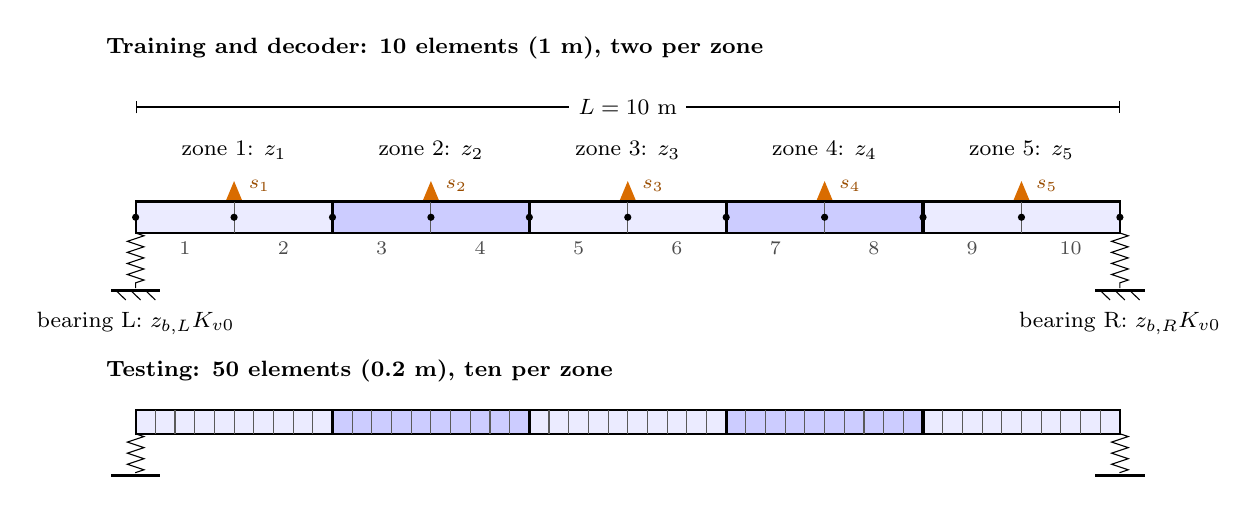
\begin{tikzpicture}[>=Stealth,font=\small,x=1.25cm,y=1cm]
  % ---- model used for training (decoder): 10 elements, 5 zones ----
  \node[anchor=west,font=\footnotesize\bfseries] at (-0.4,2.35) {Training and decoder: 10 elements (1~m), two per zone};
  \foreach \i/\c in {0/blue!8,1/blue!20,2/blue!8,3/blue!20,4/blue!8}{
    \fill[\c] (2*\i,0) rectangle (2*\i+2,0.4);
    \node[font=\footnotesize] at (2*\i+1,1.05) {zone \the\numexpr\i+1\relax: $z_{\the\numexpr\i+1\relax}$};
  }
  \draw[thick] (0,0) rectangle (10,0.4);
  \foreach \x in {1,3,5,7,9} \draw[gray!70!black] (\x,0) -- (\x,0.4);
  \foreach \x in {2,4,6,8} \draw[very thick] (\x,0) -- (\x,0.4);
  \foreach \x in {0,...,10} \fill (\x,0.2) circle (1.3pt);
  \foreach \e in {1,...,10} \node[font=\scriptsize,gray!60!black] at (\e-0.5,-0.2) {\e};
  \foreach \x/\k in {1/1,3/2,5/3,7/4,9/5}{
    \fill[orange!85!black] (\x-0.08,0.42) -- (\x+0.08,0.42) -- (\x,0.66) -- cycle;
    \node[font=\scriptsize,orange!60!black,anchor=west] at (\x+0.05,0.6) {$s_{\k}$};
  }
  \draw[|-|] (0,1.6) -- (10,1.6) node[midway,fill=white,font=\footnotesize] {$L=10$~m};
  \foreach \x/\lab in {0/{L},10/{R}}{
    \draw[decorate,decoration={zigzag,segment length=4,amplitude=3}] (\x,0) -- (\x,-0.7);
    \draw[thick] (\x-0.25,-0.73) -- (\x+0.25,-0.73);
    \foreach \h in {-0.2,-0.05,0.1} \draw (\x+\h,-0.73) -- (\x+\h+0.1,-0.85);
    \node[font=\footnotesize,anchor=north] at (\x,-0.88) {bearing \lab: $z_{b,\lab}K_{v0}$};
  }
  % ---- model used for testing: 50 elements ----
  \node[anchor=west,font=\footnotesize\bfseries] at (-0.4,-1.75) {Testing: 50 elements (0.2~m), ten per zone};
  \fill[blue!8] (0,-2.55) rectangle (2,-2.25); \fill[blue!20] (2,-2.55) rectangle (4,-2.25); \fill[blue!8] (4,-2.55) rectangle (6,-2.25);
  \fill[blue!20] (6,-2.55) rectangle (8,-2.25); \fill[blue!8] (8,-2.55) rectangle (10,-2.25);
  \draw[thick] (0,-2.55) rectangle (10,-2.25);
  \foreach \k in {1,...,49} \draw[gray!70!black] (\k*0.2,-2.55) -- (\k*0.2,-2.25);
  \foreach \x in {2,4,6,8} \draw[very thick] (\x,-2.55) -- (\x,-2.25);
  \foreach \x in {0,10}{
    \draw[decorate,decoration={zigzag,segment length=4,amplitude=3}] (\x,-2.55) -- (\x,-3.05);
    \draw[thick] (\x-0.25,-3.08) -- (\x+0.25,-3.08);
  }
\end{tikzpicture}
\caption{Description of the revised parameterization representing a short-span bridge supported on vertical elastic bearings. Top: coarse discretization used for train/validation, with ten Euler--Bernoulli elements (numbered; dots mark the nodes). Bottom: finer discretization used to generate the test data, with 50 elements. Five accelerometers ($s_1,\dots,s_5$) are placed at the centers of
the zones.}
\label{fig:bridge}
\end{figure}

\begin{table}[H]
	\centering\small
	\caption{Nominal values of the revised case study.}
	\label{tab:specs}
	\footnotesize
	\begin{tabular}{p{3.0cm}p{6.6cm}}
		\toprule
		Item & Value \\
		\midrule
		Deck & Reinforced concrete slab, span $L=10$~m, width $B=11.6$~m, depth $h=0.77$~m \\
		Concrete & elastic modulus $E=34.85$~GPa \\
		Mass & 31\,301~kg/m  \\
		Bending stiffness & $EI=1.54\times10^{10}$~N\,m$^2$, with $I=Bh^3/12$ \\
		Bearings & Vertical springs, $K_{v0}=9.5\times10^{6}$~kN/m each. \\
%		Discretization & 10 elements (training and decoder); 50 elements (test set B)\\
		\bottomrule
	\end{tabular}
\end{table}

%\begin{table}[H]
%\centering\small
%\caption{Nominal values of the revised case study and their origin.}
%\label{tab:specs}
%\footnotesize
%\begin{tabular}{p{3.0cm}p{6.6cm}p{5.0cm}}
%\toprule
%Item & Value & Origin \\
%\midrule
%Deck & reinforced concrete slab, span $L=10$~m, width $B=11.6$~m, depth $h=0.77$~m & bridge S10, Moliner et al.\ (2017), Table 2 \\
%Elastic modulus & $E=3.4849\times10^{10}$~Pa & Moliner et al.\ (2017), Table 3 \\
%Mass & 31\,301~kg/m (including ballast, sleepers and rails) & Moliner et al.\ (2017), Table 2 \\
%Bending stiffness & $EI=1.54\times10^{10}$~N\,m$^2$, with $I=Bh^3/12$ & from the values above \\
%Bearings & vertical springs, $\kappa=0.05$: $K_{v0}=9.5\times10^{6}$~kN/m each; free end rotations & $\kappa$: Moliner et al.\ (2017); range of
%commercial bearings and free rotations: Erduran et al.\ (2022) \\
%Discretization & 10 elements (training and decoder); 50 elements (test set B) & this work \\
%\bottomrule
%\end{tabular}
%\end{table}

%\begin{action}
%New FE model of the bridge on elastic bearings \lines{xx--yy}, with Fig.~\tbd{x} (Fig.~\ref{fig:bridge}) and
%Table~\tbd{x} (Table~\ref{tab:specs}).
%\end{action}

% -----------------------------------------------------------------------------
\begin{rcomment}{3}
Methodology. Another limitation is the damage parametrization presented as a ``local'' loss of stiffness distributed within an element of a specific length. Considering the type of the bridge, this type of damage parametrization is not realistic, neither for steel bridges nor for RC. This point seems particularly important as the novelty of the proposed
methodology is presented as capturing the interconnectedness of damage scenarios. I recommend, in line with the comment above, including the support conditions in the formulation, which can enable to detect damage observed there.
\end{rcomment}

\begin{response}
We have revised the formulation in two ways.

\textit{Support conditions.} As recommended, the support conditions are now part of the formulation: the elastic bearings
are represented by vertical springs at both ends of the deck, each with its own stiffness reduction factor (R2.2,
Fig.~\ref{fig:bridge}), so that damage at the supports can be identified.

\textit{Damage parameterization.} The deck is a reinforced concrete slab, in which the main damage mechanism that affects the modal response is flexural cracking.
Cracking does not occur at a single section: in a cracked region, several cracks appear at short spacing, and the bending stiffness is reduced over a certain length.
Even for a single crack, the reduction of the bending stiffness extends about 1.5 times the depth of the beam on each side of the crack~\cite{sinha2002simplified}, i.e., about 2.3~m for the present slab ($h=0.77$~m), which is comparable to the 2~m length of each damage zone.
Therefore, we represent the damage as a reduction of the effective bending stiffness of each zone, as in vibration-based FE model updating~\cite{teughels2002damage} and in the dynamic analysis of cracked slab bridges~\cite{moliner2017dynamic}.
The lower bound $z_{\text{lb}}=0.45$ corresponds to severe cracking, since a fully cracked section keeps about 20--30\% of the uncracked bending stiffness for usual reinforcement ratios.
The stiffness factor of a bearing represents a loss of vertical support stiffness, e.g., due to the deterioration of the elastomer or of its bedding.
The stiffening of the bearings with aging~\cite{erduran2022effect} is not considered, and we now mention it as a limitation. 
%To check this representation when the actual damage is concentrated, the damage of every damaged zone in test set B is imposed on a group of contiguous elements of a 50-element model, from one
%element (0.2~m) to the whole zone (2.0~m), with the same equivalent stiffness of the zone (R1.5, Eq.~\eqref{eq:localized}).
%The model used in training cannot represent this localization.
The latent space now contains seven variables, corresponding to the stiffness factors of (i) the five zones along the bridge deck and (ii) the two bearings (left and right). 
The new design of experiments (R1.6, Table~\ref{tab:doe}) focuses on healthy structures and localized damage, i.e., damage at one, two or three of these seven locations, and it also includes damage at four or more locations and samples drawn uniformly over the whole parameter space. 
%The Gaussian copula captures the dependencies between these variables, e.g., between adjacent zones and between an end zone and its bearing, which can partly compensate each other. 
%\tbd{VAE results for the bearings (benchmarks P4, P5 and P9).}
\end{response}

%\begin{action}
%New parametrization with zone and bearing stiffness factors \lines{xx--yy}; localized damage in the test data
%\lines{xx--yy}.
%\end{action}

% -----------------------------------------------------------------------------
\begin{rcomment}{4}
Methodology. The numerical case study, 5-elements simply supported beam is too simplistic. I would recommend at least
considering a more realistic case and testing the proposed method on a lab scale beam.
\end{rcomment}

\begin{response}
We have revised the proposed numerical case study to account for various aspects that make it more realistic:
\begin{enumerate}[leftmargin=*,label=(\arabic*)]
\item We employ a new parameterization of a single-span bridge, discretized into 10 Euler--Bernoulli elements and supported on elastic bearings represented by vertical springs at both ends (R2.2).
\item We account for modeling error in the form of mass perturbations (R3.1) that represent a lack of knowledge (uncertainty) about the true system properties. 
\item The design of experiments has been updated to identify localized damage at one single component of the structure, including the bearings, in addition to the multi-zone, distributed damage considered in the original manuscript.
\item We generate the test data using a finer spatial discretization (50 elements), to account for the simplifications in modeling large, complex structural systems with many DOFs.

\item An additional test dataset has been created to explore the ability of the method to identify out-of-distribution scenarios, which correspond to equivalent stiffness reductions applied to a reduced subregion of the affected zone.
\end{enumerate}
The validation on a laboratory-scale beam is not included in this revision.
We now state it clearly as a limitation of the
present work and propose the validation with data from an experimental benchmark as future work  (Section ``Conclusions and future work'').
\end{response}

%\begin{action}
%New case study \lines{xx--yy}; limitation and future work stated in the conclusions \lines{xx--yy}.
%\end{action}

% =============================================================================
\section{Reviewer \#3}
% =============================================================================

\begin{rcomment}{}
In this manuscript, a novel probabilistic machine learning framework is presented for vibration-based damage
identification in civil infrastructure. The SHM approach employs a physics-informed Gaussian copula variational
autoencoder. The effectiveness of the framework is explored in detail and validated under various damage scenarios
using synthetic, noise-contaminated data of a simply supported bridge. The manuscript contains novel theoretical
developments that are worth publishing. Before publication, the following issues have to be addressed.
\end{rcomment}


% -----------------------------------------------------------------------------
\begin{rcomment}{1}
In Bayesian finite element model updating, the discrepancy between the physical structure and the parameterized
mathematical model (i.e., modeling error) dominates over sensor noise. The current validation assumes a perfectly known
baseline mass matrix and attributes all dynamic discrepancies to stiffness reductions (which are updated in the process)
and artificial Gaussian noise. To demonstrate the robustness of the PI-GCVAE, the authors must explore its sensitivity
to modeling errors (e.g., small random perturbations to the mass matrix) and investigate how such unmodeled dynamics
propagate into the posterior uncertainty bounds for the stiffness reduction factors.
\end{rcomment}

\begin{response}
We agree with the reviewer. In the revised study, the mass matrix is no longer perfectly known.
As described in R1.2, we have included a random perturbation of the mass of each element of the FE model, Eq.~\eqref{eq:modeling_error}, which represents the modeling error.
The perturbed (true) mass values are used to generate the train, validation and test datasets.
These true values are hidden: they are not known by the physics-informed VAE, which is fed with the nominal values, considered the known, inexact system properties 
Hence, during training, the embedded eigenvalue solver uses the nominal mass matrix. 

Together with the mass perturbation, we also account for discretization error by considering a finer discretization in the test dataset compared to that used for train/validation, which introduces additional modeling error. 

These discrepancies introduce an additional source of uncertainty, besides the measurement noise, which is propagated to the estimated posterior of the stiffness factors.
In the section ``Implementation'' of the revised manuscript, we now explain modeling error in detail as part of the data generation process. 

\end{response}



% -----------------------------------------------------------------------------
\begin{rcomment}{2}
In the ``Sensitivity to $\gamma$ hyperparameter and model selection'' section, the hyperparameter $\gamma$, which
balances the data likelihood and the prior regularization, is calibrated based on the performance of the model on the
test dataset. This approach compromises the independence of the test set and results in overly optimistic performance
estimates. The optimal value of $\gamma$ must be selected using only the validation dataset. The authors need to
correct this methodological flaw and subsequently report the unbiased performance metrics on the completely unseen test
set.
\end{rcomment}

\begin{response}
In the submitted manuscript, $\gamma$ was selected with the results on the test dataset.
In the revised manuscript, we now rescale the loss functions with the variance of the data error. 
Under this calibration, we do not need the weight component $\lambda$ and can by asigning $\gamma= 1$ we obtain adequate results. 
%In the revised manuscript, $\gamma$ is no longer tuned: we fix $\gamma=1$, and the test dataset takes no part in the training or in the selection of the model.
%This is possible because we now calibrate the data terms of the loss function with the variance of their errors.
%The loss function of the submitted manuscript (Eqs.~(10)--(12)) is:
%\begin{equation*}
%\mathcal{L}_{\text{ELBO}}(\bm\theta)\approx\mathcal{L}_{\text{freq}}(\bm\theta)+\lambda\,\mathcal{L}_{\text{MAC}}(\bm\theta)+\gamma^2\mathcal{L}_{\text{PDF}}(\bm\theta),
%\end{equation*}
%\begin{equation*}
%\begin{aligned}
%\mathcal{L}_{\text{freq}}(\bm\theta)&=\frac{1}{N_{\text{train}}\cdot H}\sum_{i=1}^{N_{\text{train}}}\sum_{h=1}^{H}\big(\log\mathbf{f}_{i}-\log\hat{\mathbf{f}}_{i}^{h}\big)^{2},\\
%\mathcal{L}_{\text{MAC}}(\bm\theta)&=\frac{1}{N_{\text{train}}\cdot H\,n_{m}}\sum_{i,h,j}\big(1-\mathrm{MAC}_{j}(\bm\Phi_{i},\hat{\bm\Phi}_{i}^{h})\big).
%\end{aligned}
%\end{equation*}
%In that version, the data terms were not scaled: their relative weight was fixed empirically ($\lambda=10$), and their balance with the PDF term had to be tuned with $\gamma$.

In the revised manuscript, each squared discrepancy is divided by a scaling constant proportional to the variance of the error in the observations, and the weight $\lambda$ is no longer needed:
\begin{equation}
\mathcal{L}_{\text{ELBO}}(\bm\theta)\approx\mathcal{L}_{\text{freq}}(\bm\theta)+\mathcal{L}_{\text{MAC}}(\bm\theta)
+\gamma^2\mathcal{L}_{\text{PDF}}(\bm\theta),
\label{eq:loss}
\end{equation}
\begin{equation}
\begin{aligned}
\mathcal{L}_{\text{freq}}(\bm\theta)&=\frac{1}{N_{\text{train}}\cdot H}\sum_{i=1}^{N_{\text{train}}}\sum_{h=1}^{H}
\sum_{j=1}^{n_m}\frac{\big(\log f_{i,j}-\log\hat f_{i,j}^{h}\big)^2}{2\,\sigma_{f,j}^2},\\
\mathcal{L}_{\text{MAC}}(\bm\theta)&=\frac{1}{N_{\text{train}}\cdot H}\sum_{i,h,j}
\frac{1-\mathrm{MAC}_j\big(\bm\Phi_i,\hat{\bm\Phi}_i^{h}\big)}{2\,\sigma_{\Phi,j}^2},
\end{aligned}
\label{eq:nll}
\end{equation}
where $\sigma_{f,j}^2$ and $\sigma_{\Phi,j}^2$ are the variances of the errors of the $j$-th logarithmic frequency and of the $j$-th mode shape.
These variances include the two sources of error of the measurements, i.e., the measurement noise and the modeling error (R1.2, R3.1).
Both errors are independent, so their variances add:
\begin{equation}
\sigma_{f,j}^2=\big(\sigma_{f,j}^{\text{noise}}\big)^2+\big(\sigma_{f,j}^{\text{model}}\big)^2,\qquad
\sigma_{\Phi,j}^2=\big(\sigma_{\Phi,j}^{\text{noise}}\big)^2+\big(\sigma_{\Phi,j}^{\text{model}}\big)^2.
\label{eq:var_sum}
\end{equation}
The variance of the measurement noise is known, because we impose it when generating the data (e.g., 2.5\% for the natural frequencies).
In contrast, the variance of the modeling error is not known a priori.
Therefore, before the training phase, we run additional simulations to estimate it: we generate 6,000 extra structures with the same design of experiments and new random mass perturbations, Eq.~\eqref{eq:modeling_error}, and we compute their modal data with both the perturbed (true) and the nominal mass values, for the same stiffness factors $\z$.
The variance of the difference between both, e.g., $\log f_j^{\text{true}}-\log f_j^{\text{nom}}$, gives $\big(\sigma_{f,j}^{\text{model}}\big)^2$, and similarly for the mode shapes.
These extra simulations are not part of the train, validation or test datasets.
%As in the submitted manuscript, $\mathcal{L}_{\text{PDF}}$ is the logarithmic probability of the posterior samples under the estimated copula, i.e., minus the entropy of the approximate posterior, which is now computed in closed form (R3.7).
The justification of this scaling is simple.
For a measurement with Gaussian error of variance $\sigma^2$, the negative log-likelihood is the squared error divided by $2\sigma^2$, plus a constant.
Hence, the scaled data terms are the negative log-likelihood of the measurements, which has two consequences:
\begin{itemize}[leftmargin=*]
\item Each measured quantity is weighted according to its accuracy: an accurate measurement has a larger weight than a noisy one. This replaces the empirical weight $\lambda$.
\item With $\gamma=1$, Eq.~\eqref{eq:loss} is the negative ELBO (up to a constant, for the uniform prior), whose minimizer is the Bayesian posterior. Values $\gamma<1$ and $\gamma>1$ artificially narrow and widen the posterior, respectively.
\end{itemize}
Therefore, $\gamma=1$ is the natural choice, and it is fixed before the training.
The trained model is selected on the validation dataset: we keep the weights with the lowest validation negative ELBO, and the learning rate and the stopping of the training follow the same criterion.
% [ln z omitted in this revision, kept for later] The marginal family is compared with the same validation negative ELBO (R1.4).
The test dataset takes no part in these criteria, and the performance metrics on it are reported in Table~\ref{tab:metricsB} (R1.3).

To show the effect of $\gamma$, Appendix~\ref{app:gamma} includes a sensitivity analysis in which the model is retrained with other values of $\gamma$.
This analysis is only illustrative, and it is not used to select $\gamma$.
\end{response}
%\authornote{(i) Gamma study complete (six values, all converged); Appendix metrics computed from Val\_predicted\_props with the log-normal marginals of the model (scratchpad gamma\_val\_metrics.py), not with the truncated-Gaussian equations of R1.3. (ii) The submitted
%manuscript reports $\gamma=0.30$ (confirmed with manuscript\_old.tex and the archived run Beta0.3), and its selection
%relied on MSE, MAE and coverage values affected by the array-shape error described in R1.3. (iii) In the implementation, the likelihood of the frequencies also includes the small mean and the weak correlation of their errors, estimated by the same simulation. }
% (iv) During
% development we inspected test-set results of several marginal families, and the idea of working in $\ln z$ came from best
% fits to the exact marginals of test set A. The criterion written here is validation-only, but we cannot claim that the
% test sets were seen only once or call the metrics fully unbiased; decide how to state this.
%}

%\begin{action}
%Section ``Sensitivity to $\gamma$ hyperparameter and model selection'' rewritten \lines{xx--yy}.
%\end{action}

% -----------------------------------------------------------------------------
\begin{rcomment}{3}
Within the Bayesian setting, the posterior is heavily dependent on the choice of the prior $p(\z)$. The formulation
assumes a bounded uniform prior $\mathcal{U}[0.5,1.0]$. At the same time, the synthetic training dataset is generated
by uniformly sampling the same space. In actual SHM applications, severe damage is highly improbable; thus, a realistic
prior should strongly penalize large reductions in stiffness. The authors should clarify the distinction between the
generative sampling density used for training (which might be uniform to prevent class imbalance) and the theoretical
Bayesian prior incorporated in the ELBO loss. Can the current framework accommodate an informative, non-uniform prior
while training on uniform data? A brief discussion on this decoupling is necessary.
\end{rcomment}

\begin{response}
We agree with the reviewer that the prior has a strong influence on the posterior, and that severe damage is less probable than the healthy state and mild damage.
In this work, we assume a uniform prior, $p(\z)=\mathcal{U}[z_{\text{lb}},1]^{D}$, for the following reasons.

First, the available prior knowledge is already included through the bounds of the uniform prior.
The lower bound $z_{\text{lb}}=0.45$ (i.e., a maximum loss of stiffness of 55\%) removes the extremely severe damage states, which are the least probable ones.
Besides, these states are not the target of the method, since we aim to identify damage at an earlier stage.

Second, we do not have reliable information on the shape of the prior distribution within these bounds.
We may know that some values are less probable than others, but not how this probability is distributed: should we assume a Gaussian, an exponential, or another distribution? With which mean and variance?
Any of these choices would introduce subjective assumptions that bias the posterior without a solid basis.
Therefore, we adopt the most general case, i.e., the one with the least prior knowledge.
The uniform distribution is the least informative (maximum entropy) distribution over a bounded interval, and it is the common choice when no prior information is available.

In addition, the uniform prior keeps the training simple: the prior term of the ELBO, $-\mathbb{E}_q[\log p(\z)]$, is constant and vanishes from the loss.
The framework could accommodate an informative prior by adding this term to the loss, estimated with the same posterior samples, without changing the architecture or the training data.
However, this requires a prior with a known and tractable density (e.g., a truncated Gaussian), whose shape and parameters we cannot justify for the present problem.

Finally, note that the prior is independent of the distribution of the training data (design of experiments, R1.6), which only determines the observations from which the encoder learns.
\end{response}
\authornote{optional: demonstrate an informative prior on one benchmark.}

\begin{action}
No change is required in the manuscript.
\end{action}

% -----------------------------------------------------------------------------
\begin{rcomment}{4}
The identification relies on the first 5 modes to estimate damage in a 5-element beam. The accuracy of Bayesian
parameter estimation is fundamentally dictated by the information content of the measured data. While higher modes
offer better spatial resolution for localized damage, they are increasingly contaminated by measurement noise. A brief
sensitivity analysis or discussion of how the number of modes used affects parameter identifiability and the width of
the posterior uncertainty bounds is needed. How does the proposed VAE handle the transition to a severely ill-posed
scenario when fewer modes are available?
\end{rcomment}

\begin{response}
We agree with the reviewer: the information contained in the measured data determines the accuracy and the uncertainty of the estimates.

First, the revised case study already represents a situation of limited information.
The FE model has 10 elements for training and 50 elements for testing (R1.1), and the damage condition is described by seven stiffness factors (R2.2).
However, the measurements are still limited to five sensors and the first five modes, as in the original manuscript.

Second, to extend the analysis of data scarcity, we have trained the model assuming that only the first three modes are properly identified.
The sensors, damage scenarios, noise levels, likelihood calibration (R3.2) and training settings are the same as with five modes.
With fewer modes, the measured data are less sensitive to the stiffness of each component.
Therefore, we expect the estimated posteriors to become wider, i.e., more uncertain, instead of wrongly confident.
\tbd{Metrics on the test dataset with five and three modes: MAE, $C(0.95)$, MACE and mean width of the 95\% intervals.}

Fig.~\tbd{x} compares the estimated and the exact posteriors of a benchmark scenario with five and three modes (corner plots), and Fig.~\tbd{y} shows the marginal posteriors (violin plots) of representative test scenarios with both setups.
\tbd{Figures and short discussion: wider posteriors with three modes, close match with the exact posterior.}
\end{response}
%% Previous version (exact posteriors of five measurement setups, 06Nov data set), kept for reference:
%\tbd{see the backup response_letter_before_R34_modes_*.tex}

\begin{action}
New paragraph and figures on the effect of the number of identified modes \lines{xx--yy}.
\end{action}

% -----------------------------------------------------------------------------
\begin{rcomment}{5}
The readability of the manuscript would benefit from a dedicated flowchart illustrating the synthetic dataset
generation process (parameter sampling, forward eigenvalue solution, noise injection), distinguishing clearly between
the offline training phase and the online inference phase.
\end{rcomment}

\begin{response}
We agree, and we added the flowchart of Fig.~\ref{fig:flowchart}, which distinguishes three stages:
\begin{itemize}[leftmargin=*]
\item \emph{Offline, synthetic data generation.} The damage states are sampled with the design of experiments (R1.6);
each one is combined with a new as-built structure (random mass distribution, R1.2), its natural frequencies and mode
shapes are computed by solving the FE eigenvalue problem (with the FE model of the decoder for the training and
validation data, and with a refined FE model with localized damage for the test data, R1.5), and measurement noise is
added at the sensors.
\item \emph{Offline, physics-informed training.} The encoder maps the modal data to the Gaussian copula posterior; its
samples are passed through the embedded eigenvalue solver, and the negative ELBO (calibrated likelihood and entropy) is
minimized. The true damage states are never used in the loss.
\item \emph{Online, damage identification.} The trained encoder maps the measured modal data of the structure to the
posterior of the stiffness factors in a single forward pass, without solving the FE model, which gives the damage
assessment (posterior mean, credible intervals and healthy or damaged classification, R1.6).
\end{itemize}
\end{response}

\begin{figure}[H]
\centering
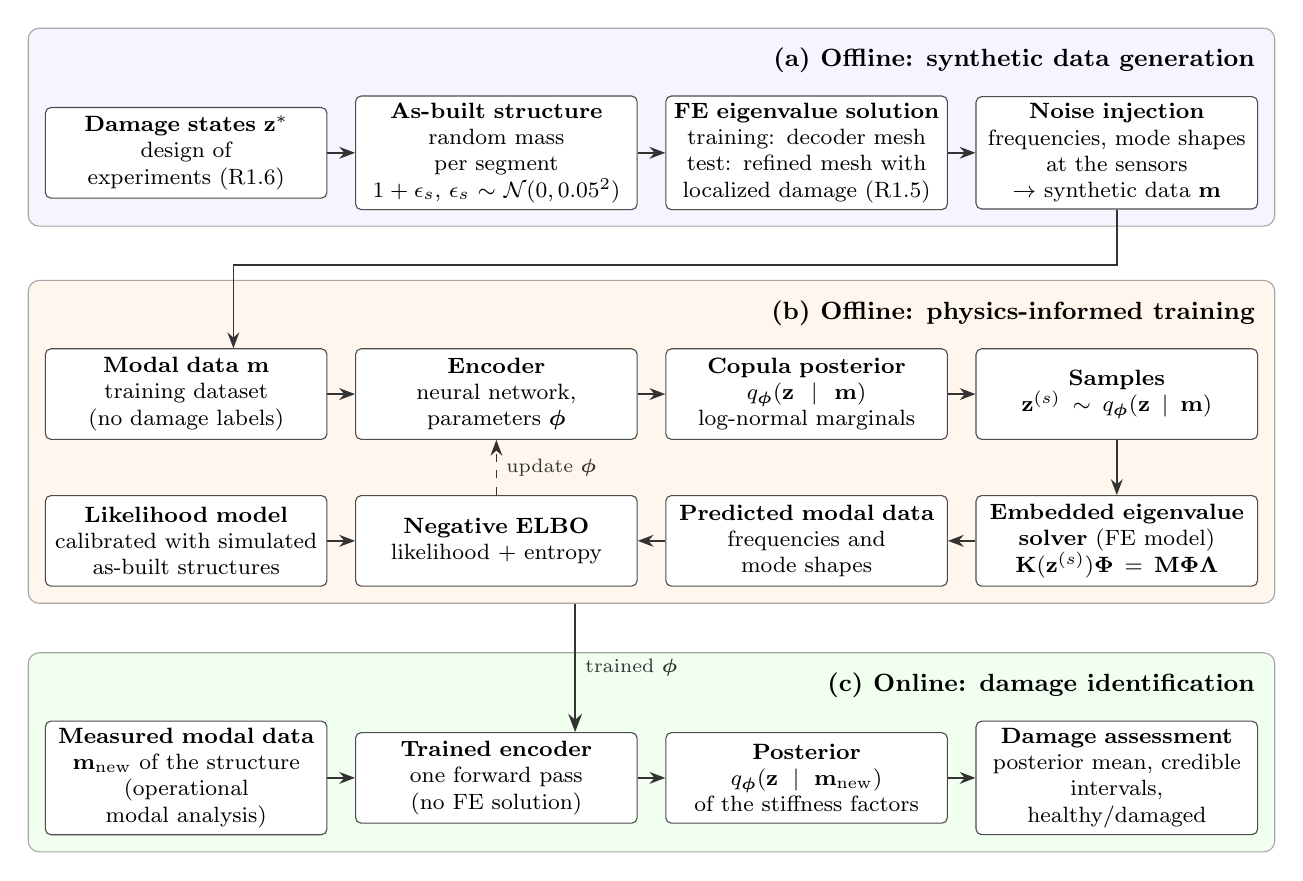
\begin{tikzpicture}[>=Stealth,font=\footnotesize,node distance=4mm and 3.5mm,
  box/.style={draw=black!70,rounded corners=2pt,align=center,fill=white,inner sep=2.5pt,minimum height=1.15cm,text width=3.4cm,execute at begin node={\hyphenpenalty=10000\relax\exhyphenpenalty=10000\relax}},
  arr/.style={->,semithick,black!80},
  ttl/.style={font=\bfseries\small,anchor=south east,inner sep=1pt},
  panel/.style={draw=black!35,rounded corners=4pt,inner sep=6pt}]
% ------------------------------------------------------------------ (a) data generation
\node[box] (doe) {\textbf{Damage states} $\z^*$\\design of experiments (R1.6)};
\node[box,right=of doe] (ab) {\textbf{As-built structure}\\random mass per segment\\$1+\epsilon_s$, $\epsilon_s\sim\mathcal{N}(0,0.05^2)$};
\node[box,right=of ab] (fe) {\textbf{FE eigenvalue solution}\\training: decoder mesh\\test: refined mesh with\\localized damage (R1.5)};
\node[box,right=of fe] (noise) {\textbf{Noise injection}\\frequencies, mode shapes\\at the sensors\\$\to$ synthetic data $\m$};
\node[ttl] (ta) at ([yshift=2.5mm]noise.north east) {(a) Offline: synthetic data generation};
\draw[arr] (doe)--(ab); \draw[arr] (ab)--(fe); \draw[arr] (fe)--(noise);
% ------------------------------------------------------------------ (b) training
\node[box,below=19mm of doe] (m) {\textbf{Modal data} $\m$\\training dataset\\(no damage labels)};
\node[box,right=of m] (enc) {\textbf{Encoder}\\neural network,\\parameters $\bm\phi$};
\node[box,right=of enc] (q) {\textbf{Copula posterior}\\$q_{\bm\phi}(\z\mid\m)$\\log-normal marginals};
\node[box,right=of q] (samp) {\textbf{Samples}\\$\z^{(s)}\sim q_{\bm\phi}(\z\mid\m)$};
\node[box,below=7mm of samp] (eig) {\textbf{Embedded eigenvalue}\\\textbf{solver} (FE model)\\$\mathbf{K}(\z^{(s)})\bm\Phi=\mathbf{M}\bm\Phi\bm\Lambda$};
\node[box,left=of eig] (pred) {\textbf{Predicted modal data}\\frequencies and\\mode shapes};
\node[box,left=of pred] (loss) {\textbf{Negative ELBO}\\likelihood + entropy};
\node[box,left=of loss] (cal) {\textbf{Likelihood model}\\calibrated with simulated\\as-built structures};
\node[ttl] (tb) at ([yshift=2.5mm]samp.north east) {(b) Offline: physics-informed training};
\draw[arr] (m)--(enc); \draw[arr] (enc)--(q); \draw[arr] (q)--(samp); \draw[arr] (samp)--(eig);
\draw[arr] (eig)--(pred); \draw[arr] (pred)--(loss); \draw[arr] (cal)--(loss);
\draw[arr,dashed] (loss.north) -- node[right,font=\scriptsize]{update $\bm\phi$} (enc.south);
\draw[arr] (noise.south) -- ++(0,-7mm) -| ([xshift=6mm]m.north);
% ------------------------------------------------------------------ (c) online
\node[box,below=17mm of cal] (meas) {\textbf{Measured modal data}\\$\m_{\mathrm{new}}$ of the structure\\(operational modal analysis)};
\node[box,right=of meas] (tenc) {\textbf{Trained encoder}\\one forward pass\\(no FE solution)};
\node[box,right=of tenc] (post) {\textbf{Posterior}\\$q_{\bm\phi}(\z\mid\m_{\mathrm{new}})$\\of the stiffness factors};
\node[box,right=of post] (out) {\textbf{Damage assessment}\\posterior mean, credible\\intervals, healthy/damaged};
\node[ttl] (tc) at ([yshift=2.5mm]out.north east) {(c) Online: damage identification};
\draw[arr] (meas)--(tenc); \draw[arr] (tenc)--(post); \draw[arr] (post)--(out);
% ------------------------------------------------------------------ panels
\begin{scope}[on background layer]
\node[panel,fill=blue!4,fit=(ta)(doe)(noise)] (pa) {};
\node[panel,fill=orange!7,fit=(tb)(m)(samp)(eig)(cal)] (pb) {};
\node[panel,fill=green!6,fit=(tc)(meas)(out)] (pc) {};
\end{scope}
\draw[arr,thick] ([xshift=10mm]tenc.north |- pb.south) -- node[right,font=\scriptsize]{trained $\bm\phi$} ([xshift=10mm]tenc.north);
\end{tikzpicture}
\caption{Methodology: (a) generation of the synthetic data, (b) offline training of the encoder through the embedded
eigenvalue solver, without the true damage states, and (c) online identification of a new structure with the trained
encoder.}
\label{fig:flowchart}
\end{figure}

\begin{action}
New flowchart (Fig.~\tbd{x}, Fig.~\ref{fig:flowchart}) \lines{xx--yy}.
\end{action}

% -----------------------------------------------------------------------------
\begin{rcomment}{6}
Equation 11 ($\mathcal{L}_{\mathrm{freq}}$): The notation $\mathbf{K}_{\mathrm{G}}$ in the decoder function is slightly
confusing since Eq. 5 defines $\hat{\mathbf{K}}_{\mathrm{G}}(\z)$ as the updated stiffness matrix. Please clarify if
$\mathbf{K}_{\mathrm{G}}$ refers to the baseline assembled matrix to avoid confusion with the damaged global matrix.
\end{rcomment}
\pending

% -----------------------------------------------------------------------------
\begin{rcomment}{7}
Sample size in training ($H=1$): In the ``Architecture design and training specifications'' section, it is stated that
a single sample ($H=1$) is drawn during training. While common in VAEs with large batch sizes, please briefly justify why
$H=1$ is sufficient to approximate the expectations in the ELBO loss.
\end{rcomment}

\begin{response}
In the revised implementation, we draw $H=6$ samples of the approximate posterior per observation. With batches of 256
observations, each gradient step uses 1\,536 samples. The Monte Carlo estimate of the loss is unbiased for any $H$, and
$H$ only affects the variance of the gradients. This variance is further reduced because the entropy is computed
exactly, in closed form (Eq.~\eqref{eq:loss}), so that the samples are only used for the expectation of the negative
log-likelihood. The samples are obtained with the closed-form quantile of the truncated normal distribution at the uniform
variables produced by the Gaussian copula. This expression is differentiable with respect to the encoder outputs, and it
replaces the rejection sampling of the submitted version.
% $H$ only affects the variance of the gradients. This variance is further reduced because the entropy is computed
% exactly, in closed form (Eqs.~\eqref{eq:marginal} and~\eqref{eq:loss}), so that the samples are only used for the
% expectation of the negative log-likelihood. The samples are obtained with the closed-form quantile of
% Eq.~\eqref{eq:marginal} at the uniform variables produced by the Gaussian copula. This expression is differentiable with
% respect to the encoder outputs, and it replaces the rejection sampling of the submitted version.
\end{response}
\authornote{optional: a short check of the sensitivity of the results to $H$.}

\begin{action}
Training specifications updated \lines{xx--yy}.
\end{action}

% -----------------------------------------------------------------------------
\begin{rcomment}{8}
Hardware and computational cost: Please report the hardware specifications and the approximate wall-clock time
required for the 11,000 training epochs to provide a practical sense of the computational cost of differentiating the
eigenvalue solver.
\end{rcomment}
\pending
\authornote{report the hardware and wall-clock time of the final training on the GPU server (NVIDIA Quadro GV100 and L40S GPUs; the eigenproblems are solved on the CPU in double precision), measured on an otherwise idle GPU.}

% =============================================================================
\appendix
\section{Appendix A: Sensitivity to $\gamma$ (R3.2)}
\label{app:gamma}
% =============================================================================
For $\gamma\neq1$, the minimizer of Eq.~\eqref{eq:loss} is the variational approximation of the tempered posterior $p_\gamma(\z|\m)\propto p(\m|\z)^{1/\gamma^2}\,p(\z)$.
A value $\gamma<1$ narrows the posterior (overconfident intervals), and $\gamma>1$ widens it (conservative intervals).
To document this effect, we retrained the model with $\gamma\in\{0.5,0.75,1,1.25,1.5,2\}$, with all the other settings unchanged.
Table~\ref{tab:gamma} reports the metrics of R1.3 on the validation dataset, for all the components and for the damaged ones ($z^{\text{true}}<0.95$).
Fig.~\ref{fig:gamma} shows the calibration of the damaged components and the MACE.

\begin{table}[H]
	\centering\small
	\caption{Sensitivity to $\gamma$ on the validation dataset (2,400 observations). $W_{95}$: mean width of the 95\% credible intervals.}
	\label{tab:gamma}
	\footnotesize
	\setlength{\tabcolsep}{4pt}
	\begin{tabular}{ccccccccc}
		\toprule
		& \multicolumn{6}{c}{All components} & \multicolumn{2}{c}{Damaged components} \\
		\cmidrule(lr){2-7}\cmidrule(lr){8-9}
		$\gamma$ & MSE & MAE & ALL & $C(0.95)$ & MACE & $W_{95}$ & $C(0.95)$ & MACE \\
		\midrule
		0.5 & 0.00493 & 0.0479 & 1.222 & 0.766 & 0.145 & 0.125 & 0.650 & 0.225 \\
		0.75 & 0.00511 & 0.0530 & 1.689 & 0.859 & 0.103 & 0.174 & 0.824 & 0.115 \\
		\textbf{1} & \textbf{0.00584} & \textbf{0.0607} & \textbf{1.715} & \textbf{0.895} & \textbf{0.107} & \textbf{0.216} & \textbf{0.917} & \textbf{0.040} \\
		1.25 & 0.00696 & 0.0695 & 1.658 & 0.910 & 0.123 & 0.253 & 0.957 & 0.012 \\
		1.5 & 0.00839 & 0.0787 & 1.580 & 0.913 & 0.143 & 0.286 & 0.974 & 0.043 \\
		2 & 0.01167 & 0.0963 & 1.430 & 0.909 & 0.179 & 0.340 & 0.981 & 0.074 \\
		\bottomrule
	\end{tabular}
\end{table}

\begin{figure}[H]
	\centering
	\includegraphics[width=\textwidth]{figures_final/Fig_gamma_validation.pdf}
	\caption{Sensitivity to $\gamma$ on the validation dataset: (a) coverage $C(p)$ of the damaged components; (b) MACE of all and of the damaged components, and mean width of the 95\% credible intervals.}
	\label{fig:gamma}
\end{figure}

The results show the expected effect of $\gamma$:
\begin{itemize}[leftmargin=*]
	\item The width of the credible intervals grows with $\gamma$, from 0.125 for $\gamma=0.5$ to 0.340 for $\gamma=2$.
	\item For $\gamma<1$, the posterior is overconfident: the 95\% coverage of the damaged components drops to 0.824 ($\gamma=0.75$) and 0.650 ($\gamma=0.5$). The point estimate improves (MAE of 0.048 for $\gamma=0.5$, against 0.061 for $\gamma=1$), mainly for the healthy components, whose narrower posteriors stay closer to the upper bound $z=1$.
	\item For $\gamma>1$, the intervals of the damaged components are conservative (coverage of 0.957--0.981), and the point estimate deteriorates (MAE up to 0.096).
\end{itemize}
With $\gamma=1$, the model yields the highest ALL, which rewards posteriors that are both accurate and well calibrated, and the posteriors of the damaged components are close to calibrated ($C(0.95)=0.917$, MACE of 0.040).
The slight undercoverage is typical of variational inference, which tends to underestimate the spread of the posterior.
For the healthy components, the 95\% coverage remains about 0.89 for every $\gamma\geq1$: about 11\% of their true values lie above the upper limit of the central 95\% interval, very close to the bound $z=1$.
This is an effect of using central intervals near the bound of the support, not of $\gamma$.
Therefore, the sensitivity analysis supports the value $\gamma=1$, fixed a priori, which provides the best balance between accuracy and calibration.

% =============================================================================
\section{References cited in this letter}
% =============================================================================
{\small
\renewcommand{\bibsection}{}
\setlength{\bibsep}{0.3ex}
\bibliographystyle{unsrtnat}
\bibliography{references_letter}
}

\end{document}
